
\documentclass[11pt,landscape,a4paper]{article}
\usepackage[utf8]{inputenc}
\usepackage[ngerman]{babel}
\usepackage{tikz}
\usetikzlibrary{shapes,positioning,arrows,fit,calc,graphs,graphs.standard}
\usepackage[nosf]{kpfonts}
\usepackage[t1]{sourcesanspro}
%\usepackage[lf]{MyriadPro}
%\usepackage[lf,minionint]{MinionPro}
\usepackage{multicol}
\usepackage{wrapfig}
\usepackage[top=5mm,bottom=5mm,left=5mm,right=5mm]{geometry}
\usepackage[framemethod=tikz]{mdframed}
\usepackage{microtype}
\usepackage{bbold}
\usepackage{wrapfig}
\usepackage{dsfont} % For mathbb{1}
\usepackage{amsmath}
\usepackage{amssymb}%Most mathematical symbols
\usepackage{mathtools}%Improved amsmath (includes amsmath), mostly structure
\usepackage{physics}%Physically relevant symbols
\usepackage{gensymb}

% START CHEATSHEET TEMPLATE

\usepackage[default]{raleway}
\usepackage{fontawesome}
\usepackage[T1]{fontenc}

\usepackage{hyperref}
\usepackage{enumitem}
\setlist[enumerate]{itemsep=0mm}
\usepackage{lipsum}

\usepackage{xcolor}
\definecolor{customcolor}{HTML}{b5e9ff}
\definecolor{alert}{HTML}{CD5C5C}
\definecolor{w3schools}{HTML}{4CAF50}
\definecolor{subbox}{gray}{0.60}
\definecolor{codecolor}{HTML}{00F0FF}
\colorlet{xx}{customcolor}

\usepackage{paralist}


%--------------------------Editor mode.

\usepackage
[citestyle=authoryear,
sorting=nty,	  		%Sorts bibliography by year, name, title
autocite=footnote, 		%Autocite command generates footnotes
autolang=hyphen, 		
mincrossrefs=1, 	
backend=biber]
{biblatex}

\DeclareFieldFormat{postnote}{#1}
\DeclareFieldFormat{multipostnote}{#1}
\DeclareAutoCiteCommand{footnote}[f]{\footcite}{\footcites}

\bibliography{literature}
%----------------------------------------
%--------------------------------------------------------------------------------
\usepackage{tcolorbox}

\tcbuselibrary{most,listingsutf8,minted}

\tcbset{tcbox width=auto,left=1mm,top=1mm,bottom=1mm,
right=1mm,boxsep=1mm,middle=1pt}

\newenvironment{mycolorbox}[2]{%
\begin{tcolorbox}[grow to left by=-1em,grow to right by=-1em,capture=minipage,fonttitle=\large\bfseries, enhanced jigsaw,boxsep=1mm,colback=#1!30!red,on line,tcbox width=auto, toptitle=0mm,colframe=#1,opacityback=0.7,nobeforeafter,title=#2]%
}{\end{tcolorbox}\\[0.2em]}

\newenvironment{subbox}[2]{%
\begin{tcolorbox}[capture=minipage,fonttitle=\normalsize\bfseries, enhanced jigsaw,boxsep=1mm,colback=#1!30!red,on line,tcbox width=auto,left=0.3em,top=1mm, toptitle=0mm,colframe=#1,opacityback=0.7,nobeforeafter,title=#2]\footnotesize %
}{\normalsize\end{tcolorbox}\vspace{0.1em}}

\newenvironment{multibox}[1]{%
\begin{tcbraster}[raster columns=#1,raster equal height,nobeforeafter,raster column skip=1em,raster left skip=1em,raster right skip=1em]}{\end{tcbraster}}

\newenvironment{textbox}[1]{\begin{mycolorbox}{customcolor}{#1}}{\end{mycolorbox}}

%-------------------------------
\newtcblisting{codebox}[2]{colback=codecolor!5,colframe=codecolor!80!red,listing only, 
minted options={numbers=left,style=tcblatex,fontsize=\scriptsize,breaklines,autogobble,linenos=false,numbersep=2mm},
left=4mm,enhanced,boxsep=1pt,left=2pt,right=1pt,top=0pt,bottom=0pt,
title=#2, fonttitle=\bfseries,
listing engine=minted,minted language=#1}

%--------------------------------------------------------------------------------
\newcommand{\punkti}{~\lbrack\dots\rbrack~}

\renewenvironment{quote}
               {\list{\faQuoteLeft\phantom{ }}{\rightmargin\leftmargin}%
                \item\relax\scriptsize\ignorespaces}
               {\unskip\unskip\phantom{xx}\faQuoteRight\endlist}
               

%--------------------------------------------------------------------------------
\newcommand{\bgupper}[3]{\colorbox{#1}{\color{#2}\huge\bfseries\MakeUppercase{#3}}}
\newcommand{\bg}[3]{\colorbox{#1}{\bfseries\color{#2}#3}}

\newcommand{\mycommand}[2]{{\ttfamily\detokenize{#1}}~\dotfill{}~{\footnotesize #2}\\}
\newcommand{\sep}{{\scriptsize~\faCircle{ }~}}


\newcommand{\bggreen}[1]{\medskip\bgupper{w3schools}{black}{#1}\\[0.5em]}
\newcommand{\green}[1]{\smallskip\bg{w3schools}{white}{#1}\\}
\newcommand{\red}[1]{\smallskip\bg{alert}{white}{#1}\\}

\usepackage{multicol}
\setlength{\columnsep}{4pt}

\setlength{\parindent}{0pt}
\pagestyle{empty}

\usepackage{csquotes}

\newcommand{\loremipsum}{Lorem ipsum dolor sit amet.}

% END CHEATSHEET TEMPLATE

\let\bar\overline

\definecolor{myblue}{cmyk}{1,.72,0,.38}

\def\firstcircle{(0,0) circle (1.5cm)}
\def\secondcircle{(0:2cm) circle (1.5cm)}

\colorlet{circle edge}{myblue}
\colorlet{circle area}{myblue!5}

\tikzset{filled/.style={fill=circle area, draw=circle edge, thick},
    outline/.style={draw=circle edge, thick}}

\pgfdeclarelayer{background}
\pgfsetlayers{background,main}

\everymath\expandafter{\the\everymath \color{myblue}}
\everydisplay\expandafter{\the\everydisplay \color{myblue}}

\renewcommand{\baselinestretch}{.8}
\pagestyle{empty}




\makeatletter
\renewcommand{\section}{\@startsection{section}{1}{0mm}%
                                {.2ex}%
                                {.2ex}%x
                                {\color{violet}\sffamily\small\bfseries}}
\renewcommand{\subsection}{\@startsection{subsection}{1}{0mm}%
                                {.2ex}%
                                {.2ex}%x
                                {\color{purple}\sffamily\bfseries}}
\makeatother

\def\multi@column@out{%
   \ifnum\outputpenalty <-\@M
   \speci@ls \else
   \ifvoid\colbreak@box\else
     \mult@info\@ne{Re-adding forced
               break(s) for splitting}%
     \setbox\@cclv\vbox{%
        \unvbox\colbreak@box
        \penalty-\@Mv\unvbox\@cclv}%
   \fi
   \splittopskip\topskip
   \splitmaxdepth\maxdepth
   \dimen@\@colroom
   \divide\skip\footins\col@number
   \ifvoid\footins \else
      \leave@mult@footins
   \fi
   \let\ifshr@kingsaved\ifshr@king
   \ifvbox \@kludgeins
     \advance \dimen@ -\ht\@kludgeins
     \ifdim \wd\@kludgeins>\z@
        \shr@nkingtrue
     \fi
   \fi
   \process@cols\mult@gfirstbox{%
%%%%% START CHANGE
\ifnum\count@=\numexpr\mult@rightbox+2\relax
          \setbox\count@\vsplit\@cclv to \dimexpr \dimen@-1cm\relax
\setbox\count@\vbox to \dimen@{\vbox to 1cm{\header}\unvbox\count@\vss}%
\else
      \setbox\count@\vsplit\@cclv to \dimen@
\fi
%%%%% END CHANGE
            \set@keptmarks
            \setbox\count@
                 \vbox to\dimen@
                  {\unvbox\count@
                   \remove@discardable@items
                   \ifshr@nking\vfill\fi}%
           }%
   \setbox\mult@rightbox
       \vsplit\@cclv to\dimen@
   \set@keptmarks
   \setbox\mult@rightbox\vbox to\dimen@
          {\unvbox\mult@rightbox
           \remove@discardable@items
           \ifshr@nking\vfill\fi}%
   \let\ifshr@king\ifshr@kingsaved
   \ifvoid\@cclv \else
       \unvbox\@cclv
       \ifnum\outputpenalty=\@M
       \else
          \penalty\outputpenalty
       \fi
       \ifvoid\footins\else
         \PackageWarning{multicol}%
          {I moved some lines to
           the next page.\MessageBreak
           Footnotes on page
           \thepage\space might be wrong}%
       \fi
       \ifnum \c@tracingmulticols>\thr@@
                    \hrule\allowbreak \fi
   \fi
   \ifx\@empty\kept@firstmark
      \let\firstmark\kept@topmark
      \let\botmark\kept@topmark
   \else
      \let\firstmark\kept@firstmark
      \let\botmark\kept@botmark
   \fi
   \let\topmark\kept@topmark
   \mult@info\tw@
        {Use kept top mark:\MessageBreak
          \meaning\kept@topmark
         \MessageBreak
         Use kept first mark:\MessageBreak
          \meaning\kept@firstmark
        \MessageBreak
         Use kept bot mark:\MessageBreak
          \meaning\kept@botmark
        \MessageBreak
         Produce first mark:\MessageBreak
          \meaning\firstmark
        \MessageBreak
        Produce bot mark:\MessageBreak
          \meaning\botmark
         \@gobbletwo}%
   \setbox\@cclv\vbox{\unvbox\partial@page
                      \page@sofar}%
   \@makecol\@outputpage
     \global\let\kept@topmark\botmark
     \global\let\kept@firstmark\@empty
     \global\let\kept@botmark\@empty
     \mult@info\tw@
        {(Re)Init top mark:\MessageBreak
         \meaning\kept@topmark
         \@gobbletwo}%
   \global\@colroom\@colht
   \global \@mparbottom \z@
   \process@deferreds
   \@whilesw\if@fcolmade\fi{\@outputpage
      \global\@colroom\@colht
      \process@deferreds}%
   \mult@info\@ne
     {Colroom:\MessageBreak
      \the\@colht\space
              after float space removed
              = \the\@colroom \@gobble}%
    \set@mult@vsize \global
  \fi}

\makeatother
\setlength{\parindent}{0pt}

\usepackage{cancel}
\usepackage{enumitem}

\begin{document}
\begin{multicols*}{4}
\scriptsize
\section*{Background}
$\log(x+1)\approx x$ if $|x|\ll 1$ \\
\textbf{Geometric series:} $\sum_{k=0}^nr^k=(\frac{1-r^{n+1}}{1-r})\overset{n\rightarrow\infty}{\longrightarrow}\frac{1}{1-r},$\hfill $ |r|<1$\\
\textbf{Hoeffding's inequality: } For $Z_i \in [a_i,b_i]$ i.i.d.\\ $P(\frac{1}{n}\sum_{i=1}^n Z_i - \mathbb E[Z]\geq t)\leq \exp(-\frac{2n^2t^2}{\sum_{i=1}^n(b_i -a_i)^2})$\\
\textbf{Hölder's inequality:} $||v \cdot u||_1\leq||v||_{p}||u||_{p^*}$ with $1/p+1/p^*\!=\!1$\\
\textbf{Jensen's inequality:} $f$ convex, then $f(\mathrm E[X])\leq\mathrm E[f(X)]$\\
\textbf{Markov's inequality:} $\mathrm P(X\geq a)\leq\frac{\mathrm E[X]}{a}$ for $X \geq 0\ a.s.,\ a > 0$\\
\textbf{KL Divergence:} $KL(Q || P) = \int_{-\infty}^{\infty} q(x)\log \frac{q(x)}{p(x)}dx$\\
\textbf{Entropy:} $H(X) = - \sum P(x_i)\log P(x_i) $

\textbf{For $A,B$ square:} $\det AB = \det A \cdot \det B$, $\det A^{-1} = \frac{1}{\det A }$\\
\resizebox{\linewidth}{!}{\textbf{MGF:}
$M_X \!:\!\mathbb{R}^n \!\rightarrow\! \mathbb{R}$, $M_X(t) \!=\! \mathbb{E}_X[\exp(t^T X)]$, $M_{X\!+\!Y} \!=\! M_X \!\cdot\! M_Y$}\\
\textbf{Moment Represent.:} $\mathbb E [X_1^{k_1} \cdots X_n^{k_n} ] = \frac{\partial^k}{\partial t_1^{k_1} \ldots \partial t_n^{k_n}} M_X \vert_{t=0}$\\
For $x \sim \mathcal{N}(\mu, \Sigma)$, we have $M_x(t) = \exp(t^T\mu + \frac{1}{2}t^T\Sigma t)$

%%%% DISTRIBUTIONS %%%%

\textbf{Normal:}
$p(x|\mu, \Sigma) = \frac{1}{\sqrt{(2\pi)^k\det(\Sigma)}} \exp(-\frac{1}{2}(x-\mu)^t\Sigma^{-1}(x-\mu))$\\
\resizebox{\linewidth}{!}{\textbf{KL-Divergence between $P \sim \mathcal{N}(\mu_P, \Sigma_P)$ and $Q \sim \mathcal{N}(\mu_Q, \Sigma_Q)$:}}\\ 
\resizebox{\linewidth}{!}{$KL(P||Q) = \frac{1}{2}[(\mu_Q - \mu_P)^T \Sigma_Q^{-1}(\mu_Q - \mu_P) + \text{Tr}(\Sigma_Q^{-1}\Sigma_P) - \ln \frac{|\Sigma_P|}{|\Sigma_Q|} - n]$}

\resizebox{\linewidth}{!}{\textbf{Gaussian Process:} $\sum_{i=1}^s \alpha_i F(x_i)\sim \mathcal N\ \forall \alpha_1, \ldots, \alpha_s \land x_1, \ldots, x_s$}


\textbf{Exponential:} $p(x|\lambda)=\lambda e^{-\lambda x}$\\
\textbf{Bernoulli:} $p(x|p)=p^x (1-p)^{1-x}$\\
\textbf{Binomial:} $p(x|n,p)={n\choose x}p^x (1-p)^{n-x}$\\
\textbf{Poisson:} $p(x|\lambda)=\frac{\lambda^x\exp[-\lambda]}{x!}$

Level sets: $L_f(z) = \{ x: \phi(w^Tx+b) = z\} \perp w$

Jacobi Matrix: $\frac{\partial F}{\partial x} = (\frac{\partial F_i}{\partial x_j})_{ij}$
\section*{Connectionism}
\textbf{Perceptron}\\[-.2cm]
$(\mathbf{x,\theta})\rightarrow \text{sgn}(\mathbf{x^T\theta}),\quad$  update:\hfill  $\Delta\mathbf{\theta}=\begin{cases} 
       \mathbf{0}, \quad y \cdot \mathbf{x^T\theta}\geq 0\\
       y\mathbf x, \quad \text{otherwise}
       \end{cases}$\\
Update path zig-zags since $\Delta\mathbf{\theta^T\theta}<0$ if \(\Delta \theta \not = 0\)\\
Update rule is SGD for the loss: $l(\mathbf x,y;\mathbf\theta)=\max\{0,-y\mathbf{x^T\theta}\}$\\
\underline{Lemma (Norm Growth)}: For perceptron mistakes $(\mathbf x^t, y^t)$ with induced updates $\Delta\mathbf\theta^t$, set  $\mathbf\theta^s=\sum_{t=1}^s\Delta\mathbf\theta^t$. Then by induction $||\mathbf\theta^s||^2\leq\sum_{t=1}^s||\mathbf x^t||^2$ and thus $||\mathbf x^t||\leq 1 \!\Rightarrow\! ||\mathbf\theta^s||\leq\sqrt s$

\textbf{Def (Linear Separability)}:  $\mathcal{D}$ linearly separable with margin $\gamma>0$ if $\exists \mathbf\theta \in \mathcal{S}^{d-1} :y \cdot \mathbf{x^T\theta}\geq\gamma \quad \forall(\mathbf x, y)\in\mathcal D$\\


\textbf{Novikov's convergence theorem:} For $\mathbf\theta^0 = 0$, $||\mathbf x^t||\leq 1$, and \(\gamma\)-separable \(\mathcal{D}\) the perceptron converges in at most $\gamma^{-2}$ updates. \textcolor{gray}{Proof: $||\theta^*|| \cdot  ||\theta^s|| \geq \langle \theta^*,\ \theta^s) =\sum_{t=1}^s \langle \theta^*,  \Delta\theta^t \rangle   = \sum_{t=1}^s y^t \cdot (x^t)^T \theta^* \geq s \gamma  \Rightarrow 1 \geq ||\theta^*|| \geq \gamma \sqrt{s}$}
\color{red}
\color{black}
\section*{Deep Linear Networks}
Assume $X \in \mathbb{R}^{n \times s}, Y\in \mathbb{R}^{m \times s}$ s.t. $\sum_{i=1}^s x_i = 0$, $\sum_{i=1}^s y_i = 0$ and $XX^T = I_n$ (whitening).
Then $W \overset{!}{\approx} \frac{1}{s} Y X^T$ since
\\$\arg\min_W ||Y - W X||_F = \arg\min_W ||W - \Gamma||_F^2,\quad \Gamma = \frac{1}{s}YX^T$ \\
This allows SVM-based analysis of 2-layer linear networks with \(\binom{rank(\Gamma)}{width}\) fixed points and one global minimum.
\textbf{Deep Linear Network Gradients:}\\
\resizebox{\linewidth}{!}{$\frac{1}{2}\frac{\partial ||W^L \cdots W^1x - y||_2^2}{\partial W^l} = (W^L \cdots W^{l+1})^T (W^L \cdots W^1x -y) x^T (W^{l-1} \cdots W^1)^T$} \\
\section*{Nonlinear Networks}
\color{black}
%\textbf{Rectified Linear Unit (ReLU):} $\mathbf x\mapsto (\mathbf x)_+=\max\{0,\mathbf x\}$\\

\vspace{-8pt}

\textbf{Absolute Value Unit (AbsU)}: $|z|, \quad \partial |z|=\begin{cases}  1 \quad\quad\quad z>0 \\ [-1,1] \quad z=0 \\ -1 \quad\quad z<0  \end{cases}$\\[-4pt]

\hfill $(z)_+=(z+|z|)/2$ and $|z|=2(z)_+-z=(z)_++(-z)_+$\\

\resizebox{\linewidth}{!}{\textbf{Logistic/Sigmoid unit}: $\sigma(z)=\frac{1}{1+\exp\{-z\}}, \quad$ $\sigma^{-1}(t)=\log\frac{t}{1-t}$}

\hfill $\sigma'(z)=\sigma(z)\cdot [1-\sigma(z)]=\sigma(z)\sigma(-z)$\\
\textbf{Hyperbolic Tangent}: $\tanh (z):=\frac{e^z-e^{-z}}{e^z+e^{-z}}=2\sigma(2z)-1$

\hfill $\tanh' (z)=1-\tanh^2(z)$\\[-2pt]
\textbf{GELU: } $\phi(z) = z \mathbb{P}(Z \leq z) \quad Z \sim \mathcal{N}(0,1)$

\textbf{Softmax:}
$\sigma_i^{\max}(\mathbf{x})=\frac{\exp[{x}_i]}{\sum_{j=1}^k\exp[{x}_j]}$

\hfill $\frac{\partial}{\partial x_j}\sigma^{\max}_i(\mathbf{x})= \begin{cases}\sigma_i^{\max}(\mathbf{x})[1-\sigma_i^{\max}(\mathbf{x})], & i=j \\ -\sigma_i^{\max}(\mathbf{x}) \cdot \sigma_j^{\max} (\mathbf{x}), & i\neq j
\end{cases}$\\[-5pt]

\textbf{Logistic Regression:}\\
Cross-entropy loss $(y\in\{-1,+1\})$:

\hspace{10pt} $l(\mathbf x, y; \mathbf\theta)=-\log\sigma(y\mathbf{x^T \theta})$ $\Rightarrow \nabla_{\mathbf\theta}l(\mathbf x,y; \theta)=-\sigma(-y\mathbf{x^T\theta})y\mathbf x$\\
Cross-entropy loss $(y\in\{0,1\})$: 

\hspace{10pt} $l(\mathbf x, y; \mathbf\theta)=-y\log\sigma(\mathbf{x^T\theta})-(1-y)\log(1-\sigma(\mathbf{x^T\theta}))$

\hfill $\Rightarrow \nabla_{\mathbf\theta}l(\mathbf x,y; \theta)=[\sigma(x^T \theta) - y] x$

\color{red}
\color{black}
\section*{Approximation Theory}
% universal approx def
\textbf{Weierstrass Theorem}\\
Polynomials $\mathcal P$ are dense ($||\cdot||_\infty$) in $C([a,b])\quad \forall a,b\in\mathbb{R}$

\textbf{Def. universal approx. $\mathcal{G}$:} $C(S) \subseteq \overline{\mathcal{G}(S)}\  \forall$ compact 
$ S \subseteq \mathbb{R}^n$
% universal approx thm
\textbf{Universal Approximation Theorem (1d)}:\\
Let $\sigma \in C^{\infty}(\mathbb{R}) \setminus \mathcal{P}(\mathbb{R})$. Then $H_{\sigma}^1 = \text{span}(\mathcal{G}_{\sigma}^1)$ is a universal approximator with $\mathcal{G}_{\sigma}^1=\{g: g(x) = \sigma(ax + b)\quad a,b\in\mathbb{R}\}$.

\textbf{Universal Approximation Theorem (n-d):}\\
$H_{\sigma}^n =\text{span}(\mathcal{G}^n_\sigma)$ is a universal approximator where\\ $\mathcal{G}_{\sigma}^n=\{g: g(x)=\sigma(x^T \theta + b)\ \theta\!\in\!\mathbb{R}^n, b \!\in\! \mathbb{R}\}$ \textcolor{gray}{(Pinkus)}
% universal in higher dim thm

\textbf{Activation Pattern in 1-layer ReLU Network:}\\
Activation pattern for input \(x\): \(\mathds{1}_{Wx+b>0} \in \{0,1\}^m \)\\
Input partition into cells: \(X_\kappa = \{x : \mathds{1}_{Wx+b>0} = \kappa\}\)\\
Restricted to a cell the network is affine.

\textbf{Zaslavsky (upper bound reached if \(\mathcal{H}\) in general pos.):}\\
$|\mathbb{R}^n - \mathcal{H}| \leq \sum_{i=0}^{\min \{m,n \}} {m \choose i} = R(m)$ with \(\mathcal{H}\) the \(m\) hyperplanes and $|\cdot|$ measuring the number of connected regions.

\textbf{Montufar (deep \(L\)-layer nets with width \(m > n\)):}\\
\# cells \(= R(m,L) \geq R(m) \lfloor \frac{m}{n} \rfloor^{n(L-1)}\) assuming general pos.

\textbf{Universality of ReLU/AbsU Networks:}

$\bullet$ Piecewise lin. functions are dense in $C([0,1])$\\
$\bullet$ Piecewise lin. function with $m$ pieces can be written as $g(x)=ax+b+\sum_{i=1}^{m-1}c_i(x-x_i)_+$ ($\exists$ formulation with $|x|$)\\
$\bullet$ NNs with one hidden layer of ReLU or AbsU are universal function approximators (with Pinkus even on $\mathbb R^n$)
\subsection*{Minimal Non-Linearity}
\textbf{k-Hinge Function (maxout unit)}: $g(\mathbf x)=\max_{j=1}^k\{\pmb\theta_j^T\mathbf x+b_j\}$\\
$\bullet$ Every continous piecewise linear function $f$ can be written as a signed sum of k-Hinges with $k\leq n+1$\\
\textbf{Polyhedral Set:} Intersection of half-planes (convex)\\
\textbf{Def. Polyhedral Function}: epigraph$(f)$ is polyhedral set\\
\textbf{Thm}: Every continous piecewise linear $f:\mathbb R^n \to \mathbb R$ can be written as the difference of two polyhedral functions\\
$\Rightarrow$ \textbf{Thm}: Maxout networks with two maxout units (difference of two k-Hinges) are universal $f$-approximators

\color{red}
\color{black}
%\section*{Rectified Networks}

\color{red}



\color{black}
\section*{Gradient Descent and Optimizers}
\resizebox{\linewidth}{!}{\textit{Gradient information provides direction of steepest descent:}}

\hspace{10pt} $\lim_{\eta\rightarrow0}\arg\min_{\pmb \vartheta:||\pmb\vartheta||_2=1}f(\mathbf{x};\pmb\theta +\eta\pmb\vartheta)=-\frac{\nabla_{\pmb\theta}f(\mathbf x;\pmb\theta)}{||\nabla_{\pmb\theta}f(\mathbf x;\pmb\theta)||_2}$\\
%Derivative wrt parameter in layer: $h'\circ g$\\
%Derivative wrt parameter in next layer: $(\partial h\circ g)\cdot g'$
%\resizebox{\linewidth}{!}{\textit{\subsection*{Notation}
%Network $F = F_{k:1} = F_k \circ F_{k-1} \circ ... \circ F_1$ \\
%Activations: $\mathbf z_l:=F_{l:1}(\mathbf x)=(F_l\circ F_{l-1:1})(\mathbf x)=F_l(\mathbf z_{l-1})$\\
%Jac. of $F:\mathbb R^n\rightarrow \mathbb R^m: \partial F=(\partial_{ij}F)=(\partial_i F_j): \mathbb R^n\rightarrow \mathbb R^{m\times n}$\\
%Chain rule for maps: $\partial(G\circ H)=\partial (G\circ H)\cdot\partial H$\\ 
%$\partial F = \prod_{l = k}^1\partial F_l \circ F_{l-1:1}, \ \partial F(\mathbf x)=\prod_{l = k}^1\partial F_l (\mathbf z_{l-1})$\\
%Loss: $f=l\circ F$\\

\subsection*{Gradient Descent and Newton's Method}
\textbf{Gradient Descent:}\\
\resizebox{\linewidth}{!}{Discretize gradient flow $\dot{\mathbf \theta}=\text{-}\nabla f(\mathbf \theta)$ as $\mathbf \theta_{t+1}=\mathbf \theta_t-\eta\nabla f(\mathbf \theta_t)$}

\textbf{Newton's Method}:\\
Directly jumps to minimum of 2nd order Taylor of $f$:

\hspace{15pt} $f(\mathbf{\theta+\Delta \theta})\approx f(\mathbf \theta)+\Delta\mathbf \theta^T \nabla f(\mathbf \theta)+\frac{1}{2}\Delta\mathbf \theta^T\nabla^2f(\mathbf \theta)\Delta\mathbf \theta$\\
which results in $\Delta\mathbf \theta=-[\nabla^2f(\mathbf \theta)]^{-1}\nabla f(\mathbf \theta)$. GD is recovered under isotropy assumption on the Hessian ($\nabla^2 f(\mathbf \theta)=\frac{1}{\eta}\mathrm I$)

\textbf{Batch Gradient Descent (unbiased with $\mathbb{E}[\nabla \hat{f}_\theta] = \nabla f_\theta$):}\\
Compute $\nabla \hat f_\theta = \frac{1}{r}\sum_{t=1}^r f_\theta(x_{i_t}, y_{i_t})$ where $i_t \sim \mathcal U(\{1, \ldots, s\})$.

\textbf{SGD ($r=1$) Variance Reduction Technique (SVRG):}\\
Every $T$ steps compute full gradient $\nabla_\vartheta f_{\vartheta}$. Use updates $\theta_{t+1}=\theta_t-\eta[\nabla f_{\theta_t}(x_i, y_i)-\nabla f_{\vartheta}(x_i, y_i) +\nabla_\theta f_{\vartheta}]$

\textbf{Compressed Stochastic Gradients (SignSGD):}\\
Update $\theta_{k+1} = \theta_k-\eta_k\text{sign}[\nabla f(\theta_k)(x_{i_t}, y_{i_t})]$.

\subsection*{Gradient Descent with Momentum}
\textbf{Nesterov’s Accelerated Gradient Descent:}\\
$x_{k+1} = y_{k}-\eta\nabla f(y_{k+1}) \quad y_{k} = x_k+\beta(x_k-x_{k-1}) \quad\hfill \beta \in [0,1)$

\textbf{Polyak's Heavy Ball Method:}\\
$x_{k+1} = x_k -\eta\nabla f(x_k)+\beta(x_k-x_{k-1})\quad\hfill \beta \in [0,1)$\\[-3pt]
\resizebox{\linewidth}{!}{with $x_{t+1} - x_{t} = - \eta\sum_{k=0}^t \beta^{t-k} \nabla f(x_k) \xrightarrow{t\to\infty,\ const\ \nabla f} -\frac{\eta}{1-\beta} \nabla f$}

\subsection*{Adaptive Gradient Descent}
\textbf{AdaGrad (decays LR based on 2nd moment estimate):}\\
$\theta[j]$ is updated with learning rate $\eta_{t,j} = \frac{\eta}{\gamma_{t,j} + \delta}$ where  $\gamma_{t,j}^2 = \gamma_{t-1,j}^2 + (\frac{\partial f_\theta(x_{i_t}, y_{i_t})}{\partial \theta_{t}[j]})^2$ with  $0 < \delta \approx 0$ for stability.\\
\textbf{Adam - Adaptive Moment Estimation (w. momentum):}\\
Exponential averages: $\Delta_{t+1} = \alpha \Delta_t + (1-\alpha)\nabla{f_\theta}(x_{i_t},y_{i_t})$ and $\gamma_{t+1,j}^2 = \beta\gamma_{t,j}^2 + (1-\beta)(\frac{\partial f_\theta(x_{i_t}, y_{i_t})}{\partial \theta_{t}[j]})^2$ where $\alpha, \beta \in [0,1)$\\
Update: $\theta_{t+1}[j] = \theta_{t}[j] + \frac{\eta}{\gamma_{t,j}/(1-\beta)+\delta}\frac{\Delta_{t+1,j}}{1-\alpha}$ with  $0 < \delta \approx 0$\\

\textbf{AMSGrad (fixes/ensures convergence):}\\
Adam + monotonicity $\tilde \gamma_{t+1, j} = \max(\gamma_{t+1, j}, \tilde \gamma_{t, j})$.

\subsection*{Backpropagation}
%$\nabla_{\pmb\theta_l}F=(\partial F_{k:l+1}\circ F_{l:1})\cdot(F'_l\circ F_{l-1:1}) =\partial F_{k:l+1}(\mathbf z_l)\cdot F'_l(\mathbf z_{l-1})$\\Corresponds to downstream Jacob. $\times$ local Jacob:
\textbf{Chain rule:} $\partial (G\circ F_{\pmb\theta} \circ H) = (\partial G \circ F_{\pmb\theta}\circ H)\cdot (\partial F_{\pmb\theta}\circ H)$\\
%$\nabla_{\pmb\theta_l}f(\mathbf x)=\partial(l\circ F_{k:l+1})(\mathbf z_l)\cdot F'_l(\mathbf z_{l-1})=:\pmb\xi_{l+1}\cdot F'_l(\mathbf z_{l-1})$\\
%Row vectors $\pmb\xi_{l}$ calculated through backward iteration: \\
%$\pmb\xi_{k+1}=\partial l(\mathbf z_k), \quad \pmb\xi_{l}=\pmb\xi_{l+1}\partial F_l(\mathbf z_{l-1})$\\
\textbf{Backpropagation algorithm} consists of three steps:\\
(1) forward pass computing all pre-activations $\mathbf z_l$, \\
(2) backward pass computing all $\pmb\xi_{l} = \frac{\partial L}{\partial z_l} = \frac{\partial L}{\partial z_{l+1}} \frac{\partial z_{l+1}}{\partial z_{l}}$\\
(3) local computations computing all $\frac{\partial L}{\partial W_l} = \frac{\partial L}{\partial z_l} \frac{\partial z_l}{\partial W_l}$
\subsection*{\resizebox{\linewidth}{!}{Automatic Differentiation of $f:\mathbb R^N\rightarrow\mathbb R^M$ as a DAG($V$, $E$)}}
Usually $N=\#\text{parameters}$ and $M=1$ (scalar loss).

\textbf{Forward Mode:} Chain rule from right to left (no separate forward pass). Scales in $\mathcal O(N(V+E))$.

\textbf{Reverse Mode:} Chain rule from left to right (needs sepa- \resizebox{\linewidth}{!}{rate forward pass $\Rightarrow$ more memory). Scales in $\mathcal O(M(V+E))$.}

%El.-wise function (e.g. activation fun): $\frac{\partial}{\partial \mathbf x}f(\mathbf x)=\text{diag}(f'(\mathbf x))$%\\
%ReLU wrt pre-activations: $\frac{\partial}{\partial \mathbf x}\max(0,\mathbf x)=\text{diag}(H(\mathbf x))$\\
%" \ wrt $\pmb\theta$: $\frac{\partial}{\partial \mathbf W_{ij}}\max(0,\mathbf{Wx})_k=\max(0,\text{sign}(\mathbf{W_i}^T\mathbf x))x_j\delta_{ik}$\\
%" \ wrt activ.: $\frac{\partial}{\partial \mathbf x_j}\max(0,\mathbf{Wx})_i=\max(0,\text{sign}(\mathbf W_i^T\mathbf x))\cdot W_{ij}$

\color{red}
\color{black}
\section*{Optimization Convergence Guarantees}
%\subsection*{Loss Functions}
%\textbf{Squared:} $l_\mathbf y(\pmb \nu)=\frac{1}{2}||\mathbf y -\pmb\nu||^2$,
%\textbf{0-1 loss:} $l_y(v)=\begin{cases} 0, \quad \nu=y \\ 1, \quad \text{else}\end{cases}$\\
%\textbf{Cross-entropy (multiclass):} $l_y(\nu)=-\log \nu_y$\\
%Soft target cross-entropy ($\mathbf y\in[0,1]^m$): \\
%$l_\mathbf y(\pmb \nu)=-\sum_{j=1}^my_j\log\nu_j\geq-\sum_{j=1}^my_j\log y_j=:H(\mathbf y)$\\
%Prob. loss: $l_\mathbf y(\pmb\nu)=-\log p(\mathbf y;\pmb \nu)$ (e.g. replace with isotropic Gaussian to get squared loss)\\
%\textbf{Exponential family:} $p(\mathbf y;\pmb\nu)=h(\mathbf y)\exp[\mathbf y\cdot\pmb\nu-\psi(\pmb\nu)]$, log partition/normalizing function $\psi$\\
%Can construct losses by taking distributions in the exponential family in the log prob loss andx replace $\pmb\nu$ with $h(\pmb\theta\cdot\mathbf z)$, where $\mathbf z$ is produced by a Neural Network

\subsection*{Convexity, Smoothness, and Polyak-Lojasiewicz}
\resizebox{\linewidth}{!}{\textbf{Def. Convexity:} $f(\lambda x +(1\text{-}\lambda)y)\leq \lambda f(x)+(1\text{-}\lambda)f(y) \ \forall\lambda\in[0,1]$}\\
\textbf{Def. Convexity of Diff'ble $f$:} $f(x)\geq f(y)+\nabla f(y)^T(x-y)$\\
\resizebox{\linewidth}{!}{\textbf{Def. $\mu$-Strong Convexity:} $f(x)\geq f(y)+\nabla f(y)^T(x\text{-}y)+\frac{\mu}{2}||x\text{-}y||^2$}\\
\textbf{Def. Lipschitz Smoothness:} $||\nabla f(x)-\nabla f(y)||_2\leq L||x-y||_2$\\
\resizebox{\linewidth}{!}{$L$-Smoothness implies $f(x)\leq f(y)+\nabla f(y)^T(x-y)+\frac{L}{2}||x-y||^2_2$}

\hfill \resizebox{\linewidth}{!}{\textcolor{gray}{using $f(x) - f(y) - \nabla f(y)^T (x-y) = \int_0^1 [\nabla f(y + (x-y)s) - \nabla f(y)]^T(x-y) ds$}.\hspace{30pt}}

\resizebox{\linewidth}{!}{Applied to GD we get $f(\theta - \frac{1}{L} \nabla f(\theta)) \leq f(\theta) - \frac{1}{2L} || \nabla f(\theta)||_2^2$.\hspace{10pt}}\\
\resizebox{\linewidth}{!}{\textbf{Hessian of $L$-Smooth \& $\mu$-Strongly Convex:} $\mu\mathrm I\preccurlyeq\nabla^2 f\preccurlyeq L\mathrm I$}\\
$\epsilon$-\textbf{Stationarity (approximate stationarity):} $||\nabla f(x)||_2\leq\epsilon$\\
\textbf{PL condition:}
 $\forall y\ \frac{1}{2 \mu}||\nabla f(y)||^2\geq f(y)-\min_x f(x)$\\
 implied by $\mu$-strong convexity.

\subsection*{Convergence of GD and GD with Nesterov Momentum}
\textbf{Thm. Polyak:} Given $f$ $L$-smooth and $\mu$-PL, then GD with $\eta = 1/L$, i.e. $x_{t+1} = x_t - \frac{1}{L} \nabla f(x_t)$, converges globally:

\hspace{25pt} $f(x_t) - \min_x f(x) \leq (1-\frac{\mu}{L})^t [f(x_0) - \min_x f(x)]$

\textbf{Thm. Nesterov:} Given $f$ $L$-smooth and $\mu$-strongly convex with conditioning $\kappa = \frac{L}{\mu}$ and $\beta = \tfrac{\sqrt{\kappa}-1}{\sqrt{\kappa}+1}$, then Nesterov GD converges globally: $f(x_t)-f(x^*)\leq L(1- \sqrt{\tfrac{\mu}{L}})^t\|x_0-x^*\|^2$\\

\subsection*{Convergence of Stochastic Gradient Descent}
Consider BGD with $r=1$. Then
$||\theta_t \text{-} \theta_*||^2 - \hat{\mathbb{E}}_{x,y} ||\theta_{t+1} \text{-} \theta_*||^2$ = $2 \eta_t (\theta_t \text{-} \theta_*)^T \hat{\mathbb E}_{x,y} \nabla f_{\theta_t}(x, y) - \eta_t^2 \hat{\mathbb E}_{x,y} ||\nabla f_{\theta_t}(x, y)||^2$ is positive for small enough $\eta_t$ and $(\theta_t - \theta_*)^T \nabla \frac{1}{s}\sum_{k=1}^s f_{\theta_t}(x_k, y_k) > 0$.

\textbf{Polyak Averages:} To reduce $\hat{\mathbb E}_{x,y} ||\bar{\theta}_{t+1} - \bar{\theta}_{t}||^2$ use Polyak \resizebox{\linewidth}{!}{averaging
$\bar{\theta}_{t+1}\!=\! \frac{t\cdot \bar{\theta}_t}{t+1}\!+\!\frac{\theta_{t+1}}{t+1} \! =\! \frac{-\eta_t \nabla f_{\theta_t}(x,y)}{t+1}$. Let $\eta_t \propto \frac{1}{t}$, then}\\
$\bullet$ $f$ convex: $\hat{\mathbb E}[f(\bar{\theta_t})] - f(\theta^*) \in \mathcal{O}(1/\sqrt{t})$\\
$\bullet$ $f$ $\mu$-strongly convex: $\hat{\mathbb E}[f(\bar{\theta_t})] - f(\theta^*) \in \mathcal{O}(\frac{\log t}{t})$\\
$\bullet$ $f$ $\mu$-strongly convex \& $L$-smooth: $\hat{\mathbb E}[f(\bar{\theta_t})] - f(\theta^*) \in \mathcal{O}(\frac{1}{t})$\\

\textbf{Quasi-Convergence of SGD with Constant Step Size:}\\
Let $f_\theta \!=\! \frac{1}{s} \sum_{k=1}^s f_\theta(x_k, y_k)$ be \underline{$\mu$-strongly convex} with each $\theta \mapsto f_\theta(x_k, y_k)$ being \underline{$L$-smooth} with measure of variance $\sigma^2 =\frac{1}{s}\sum_{k=1}^s||\nabla_\theta f_\theta(x_k, y_k)-\nabla_\theta f_\theta||^2$. Then for SGD with $\eta_{const} \leq1/\mu$ it holds
$\hat{\mathbb{E}}\|\theta_t-\theta^*\|^2\leq A^t\|\theta_0-\theta^*\|^2+B$
where $A=1-2\eta_{const}\mu(1-\eta_{const} L) $ and $B=\frac{\eta_{const}\sigma^2}{\mu(1 - \eta_{const} L)}$.\\

%\textbf{Gradient clipping: } To avoid exploding gradients, can bound the norm of the gradient in the update step by a threshold (e.g. when reaching a "cliff")
%\subsection*{Momentum} If gradients start going into a particular direction, keep going in that same direction (inertia in direction we had)\\
\color{black}



\color{black}
\section*{Convolutional Networks}
\subsection*{Convolution Operator}
\textbf{Integral Operator:}
$\left(Tf\right)(u)=\int_{t_1}^{t_2} H(u,t)f(t)dt$\\
\textbf{Convolution:}
$(f*h)(u):=\int_{-\infty}^{\infty} h(u - t)f(t) dt = (h * f)(u)$\\
\textbf{Discrete Convolution:} $(f*h)[u]:=\sum_{t=-\infty}^{\infty}f[t]h[u-t]$\\
\textbf{Theorem:} An operator $T$ is linear and shift-equivariant $\iff$ $T$ is a convolution $T(f) = f \ast h$ for some kernel $h$\\
\textbf{Cross-Corr.:} $(f\star h)[u]:=\sum_{t=-\infty}^{\infty}f[t]h[u+t] = (f[-\ \cdot]*h)[u]$\\
\textbf{Fourier Transform:} $(\mathcal{F}f)(u):=\int_{-\infty}^{\infty}\exp\{-2\pi itu\}f(t)dt$\\
\textbf{Convolution Theorem:} $u * v = \mathcal F^{-1}(\mathcal F u \cdot \mathcal F v)$\\
\textbf{Toeplitz Matrices}: Constant diagonals (1D convolutional kernel can be written as a Toeplitz matrix product)
\subsection*{Convolutional Neural Networks}
\textit{Exploiting translation equivariance, locality, and scale.\\
More efficient through parameter sharing and locality.} \\
\textbf{(Local) Receptive Field of $x_i^l$:} $\ \mathcal{I}_i^l:=\{j:w_{ij}^l\neq 0 \}$\\
\textbf{Sparse Backpropagation:} $\partial x_i^l/\partial x_j^{l-1}=0$, for $j\notin \mathcal{I}_i^l$\\
\textbf{Weight Sharing:} $\tfrac{\partial\mathcal{R}}{\partial h_j^l} = \sum_i\tfrac{\partial\mathcal{R}}{\partial x_i^l}\tfrac{\partial x_i^l}{\partial h_j^l}$,\,\, $h_j^l$ kernel weight\\
\textbf{Pooling 2D}: $x_{ij}^{\max}=\max\{x_{i+k,j+l}:0\leq k< r,0\leq l< r\}$\\
\textbf{2D Convolutional Layer:} ($\mathbf{X,Y}$ are of shape (c, x, y))\textbf{:}\\ $y[r][s,t]=\sum_u\sum_{\Delta s,\Delta t}w[r,u][\Delta s, \Delta t]\cdot x[u][s+\Delta s, t+\Delta t]$\\
\resizebox{\linewidth}{!}{\textbf{Output Size:} $\left\lfloor (input\_width+2pad-filter\_width)/stride \right\rfloor + 1$}\\
\textbf{Embeddings from Log-Bilinear:} $\mathbb{P}(\nu|\omega) = \tfrac{\exp(x_\omega^T y_{\nu})}{\sum_\mu \exp(x_\omega^T y_\mu)}$
\color{red}
\input{deep_gradients}
\section*{Regularization}
\color{black}
\textit{To lower generalization error but not the training error.\\
$\bullet$ informed regularization (prior knowledge)\\
$\bullet$ simplicity bias (Occam's razor)\\
$\bullet$ Bayesian averaging (ensembling, dropout)
}
\subsection*{$L_2$-Regularization / Weight Decay}

Regularized objective becomes 
$\overline{E}_\theta(S)=E_\theta(S)+\mu\Omega(\theta)$
where $\Omega(\theta) = \frac{1}{2} \sum_{l=1}^L ||W^l||_F^2 = \frac{1}{2} \sum_i \theta_i^2$ (no bias reg.) for $\theta = vec(W^1, \ldots, W^L, b^1, \ldots, b^L)$. Since $\nabla_\theta \Omega(\theta) =\mu\theta$ the GD\\ update includes weight decay: $\theta_{t+1} \!=\! (1\text{-}\eta \mu) \theta_t \text{-} \eta \nabla_\theta E_{\theta_t}$

\resizebox{\linewidth}{!}{\textbf{Spectral Analysis based on Taylor around \(\arg\min E_\theta(S)\):}}\\
$\bar E_\theta(S) \approx E_{\theta^*}(S)+\frac{1}{2}(\theta-\theta^*)^TH_E(\theta-\theta^*) + \mu \Omega(\theta) + \mathcal{O}(||\theta - \theta^*||_2^3)$ with Hessian $H_E=Q\text{diag}(\lambda_i)Q'$. By first order conditions\\ $\theta\overset{!}{=}(H_E+\mu I)^{-1}H_E\theta^*=Q\text{diag}(\frac{\lambda_i}{\lambda_i+\mu})Q'\theta^*$. Hence, along low-curvature directions ($\lambda_i \ll \mu$) the weights are shrunk.

\textbf{Constrained Optimization:}\\
Regularization objective becomes $\arg\min_{\{\theta:\norm{\theta}\leq r\}}E(\theta)$. Regularization only effective at late stages of learning.\\
Optimized using projected gradient descent:

\hspace{4pt} $\theta_{t+1}=\Pi_r[\theta_t-\eta\nabla E_{\theta_t}(S)]$ where $\Pi_r(v)=\min\left\{1,\frac{r}{\norm{v}}\right\}v$

\textbf{Ridge Regression: }Linear regression + $L_2$-regularization is termed Ridge regression with $\pmb\theta^* = (\mathbf{X}^{\intercal}\mathbf{X}+\lambda\mathrm{I})^{-1}\mathbf{X}^{\intercal}\mathbf{y}$.

\subsection*{Early Stopping}
Stop learning when loss on validation data increases. Early stopping acts as an approximate $L2$-regularizer:

\resizebox{\linewidth}{!}{\textbf{Spectral Analysis based on Taylor around \(\arg\min E_\theta(S)\):}}\\
$\nabla_\theta E_\theta(S) \approx H_E(\theta-\theta^*) + \mathcal{O}(||\theta - \theta^*||_2^2)$ w. $H_E=Q\text{diag}(\lambda_i)Q'$ giving GD update $\theta_{t+1} = \theta_t - \eta H_E(\theta_t-\theta^*) + \mathcal{O}(||\theta_t - \theta^*||_2^2$.

Hence, $\theta_{t+1} - \theta^* = (I - \eta H_E)(\theta_t-\theta^*) + \mathcal{O}(||\theta_t - \theta^*||_2^2$. Then

$\theta_t = \cancel{(I - \eta \text{diag}(\lambda_i))^t Q' \theta_0} + Q[I - (I - \eta \text{diag}(\lambda_i))^t]Q' \theta^*$

(by induction) where the first term is neglected if $\theta_0 = 0$.

Since $t \eta \text{diag}(\lambda_i) \overset{\eta \lambda_i \ll 1}{\approx} I - (I-\eta \text{diag}(\lambda_i))^t \overset{!}{=} \text{diag}(\frac{\lambda_i}{\lambda_i + \mu})$ we get $L_2$-regularization given $\eta\lambda_i \ll 1$, \underline{$\lambda_i \ll \mu$, $t=\frac{1}{\eta\mu}$}.
\subsection*{Residual Connections}
Parametrize $G_\theta(x)=x+F_\theta(x)$ with $F \approx 0$ at initialization giving Jacobian $J_G \approx I$ (good for backpropagation) and allowing weight decay toward identity. ResNets augment deep CNNs with residual connections. DenseNets further employ skip connections to all downstream layers. \\[3pt]
$\bullet$ Residual Connections adds shortcut to output\\
$\bullet$ Skip Connections concatenates shortcut to output 
\subsection*{Normalization}
Calibrate dynamic range of unit $j$ in layer $l$ (datapoint $i$):\\
\textbf{Batch Normalization ($\gamma_j^l, \beta_j^l$ are params):}\\
Normalization: $\Tilde{z}_j^l[i]=\frac{z_j^l[i]-\mu_j^l}{\sigma_j^l+ \delta} \quad 0 < \delta \approx 0, \hfill \hat{z}_j^l=\gamma_j^l+\beta_j^l\Tilde{z}_j^l$\\
Statistics: $\mu_j^l = \frac{1}{|B|} \sum_{i \in B} z_j^l [i], \hfill (\sigma_j^l)^2 = \frac{1}{|B|} \sum_{i \in B} (z_j^l [i] - \mu_j^l)^2$\\
\textbf{Layer Normalization (normal. along single instance):}\\[5pt]
Normalization:  \underline{same formula as in Batch Norm}\\[5pt]
Statistics: $\mu_j^l = \frac{1}{m_l} \sum_{j =1}^{m_l} z_j^l [i], \hfill (\sigma_j^l)^2 = \frac{1}{m_l} \sum_{j =1}^{m_l} (z_j^l [i] - \mu_j^l)^2$\\
\subsection*{Dropout}
Randomly drop subsets of units for more robustness with retention probability $\pi_i^l$ for unit $i$ in layer $l$ (input $\pi_i^0=0.8$ and hidden unit $\pi_i^{l\geq 1}=0.5$). Creates an 
\underline{exponentially large (in \#nodes) ensemble} of networks.\\[5pt]
At inference, use as an ensemble method or rescale weights $\Tilde{w}_{ij}^l\leftarrow\pi_j^{l-1}w_{ij}^l$ calibrating the net input to unit $i$.
\subsection*{Data Augmentation}
\textit{Trick to generate larger, non-i.i.d. training set}\\[5pt]
Generate virtual examples by applying transformations $\tau$ to each training example $(\mathbf{x},\mathbf{y})\mapsto (\tau(\mathbf{x}),\mathbf{y})$, e.g. 
PCA, cropping \& resizing, rotations \& reflections, etc.\\[5pt]
We can add noise to the inputs (ideally realistic noise), to the weights (regularizing effect) or to the targets (soft targets/label errors). Also helps with model robustness. 
\subsection*{Self-Supervised Training}
Pretrain a model on a (self-supervised) task (e.g. patch location prediction, image coloring, video motion prediction, predictive coding of latent states) before finetuning.\\[5pt]
\textbf{Contrastive Predictive Coding}

\begin{minipage}{.6\linewidth}
    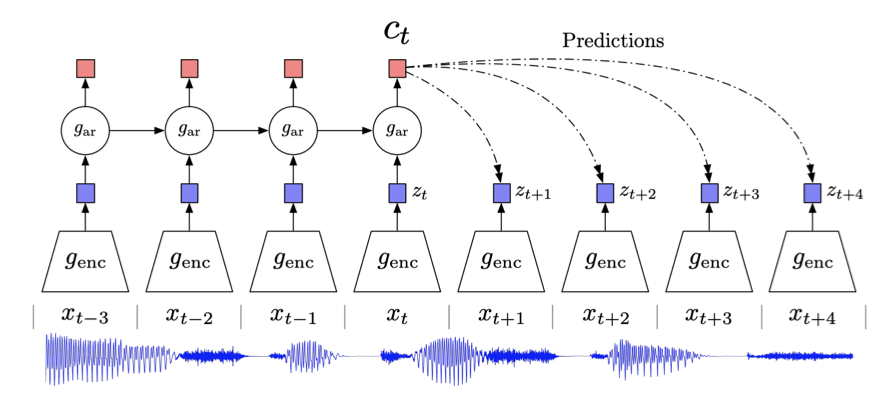
\includegraphics[width=\linewidth]{contrastive_predictive_coding.png}
\end{minipage}
\begin{minipage}{.4\linewidth}
    Maxim. density ratio\\
    $\frac{p(x_{t+1}\mid c_t)}{p(x_{t+1})} \propto e^{z_{t+1}^TWc_t}$\\
    for positive examples\\ and minimize for\\
    negative examples
\end{minipage}

\color{black}

\section*{Geometric Deep Learning}
\textbf{Group}: A set $\mathcal{G}$ with binary operation $\circ: \mathcal{G} \times \mathcal{G} \rightarrow \mathcal{G}$ s.t. \\
\underline{Closure:} $gh \in \mathcal{G}\ \forall g,h \in \mathcal G$\\
\underline{Associativity}: $(gh)f = g(hf) \,\, \forall g,h,f \in \mathcal{G}$\\
\underline{Identity:} $\exists!\ e \in \mathcal{G}$, for which $eg = ge = g\quad  \forall g \in \mathcal G$\\
\underline{Inverse:} $\forall g\ \exists!$ $g^{-1} \in \mathcal G$, s.t. $gg^{-1} = g^{-1}g = e$\\
\textbf{Group Action:} \(\otimes: G \times X \to X\) s.t. \(e(x) = x \ \land \ g(h (x)) = gh( x)\)
\resizebox{\linewidth}{!}{\textbf{Linear Group Action:} $g(\alpha x + y) = \alpha g(x) + g(y)$ with Repre-}\\
\resizebox{\linewidth}{!}{sentation $\rho: \mathcal{G} \rightarrow \mathbb{R}^{n\times n}$ s.t. $\rho(g)x = g(x) \Rightarrow \rho(gh) = \rho(g)\rho(h)$}\\
\textbf{Action on Signals:} $(\rho(h) x)(s) = x(h^{-1} s)$ where $x: \Omega \to \mathbb{R}\quad$\\
\resizebox{\linewidth}{!}{\textbf{$\mathcal{G}$-Invariance}: $f : \mathcal{X}(\Omega) \rightarrow \mathcal{Y}$ satisfies $f(\rho(g)x) = f(x)\ \forall g \in \mathcal G$}\\
\resizebox{\linewidth}{!}{\textbf{$\mathcal{G}$-Equivariance:} $f : \mathcal{X}(\Omega) \rightarrow \mathcal{X}(\Omega)$ fulfills $f(\rho(g)x) = \rho(g) f(x)$}\\
\textbf{$\mathcal{G}$-Convolution}: $(x * \theta)(g) = \int_\Omega x(u) \theta(g^{-1}u) du \quad g \in \mathcal G$\\
$(\rho(h) x * \theta)(g) = \rho(h) (x * \theta)(g) \quad (x * \rho(h)\theta)(g) = (x * \theta)(gh)$
\resizebox{\linewidth}{!}{\textbf{Smoothing for Invariance:} $(S_\mathcal{G}f)(x) = \frac{1}{|\mathcal{G}|} \sum_{g \in \mathcal{G}} f(\rho(g) (x))$}\\
\textbf{Deep Sets:} can represent any in-/equivariant function on sets using only the following two layers:\\
\underline{Invariant Layer}: $f(X) = \phi\left( \sum_{x \in X} \psi(x) \right)$ with $\phi, \psi$ learnable.\\
\underline{Equivariant Layer}: $f(X, x_i) = \phi\left( \sum_j \psi(x_j), x_i \right)$
\subsection*{Graph Neural Nets}
\textbf{Node Feature Matrix:} $X = [x_1, ..., x_n]^T \in \mathbb{R}^{n\times k}$\\
\textbf{Permutation Invariance}: $f(PX, PAP^T) = f(X, A)$\\
\textbf{Permutation Equivariance}: $f(PX, PAP^T) = Pf(X, A)$\\
\textbf{1-Hop Neighbourhood of $x_i$:} $\mathcal{N}_i = \{j: A_{i,j} \not = 0\}$\\
\textbf{E.V. GNN Layer}: $f(X, A) = [\phi(x_1, X_{(\mathcal{N}_1)}), \dots, \phi(x_n, X_{(\mathcal{N}_n)})]$ for the multiset $X_{(\mathcal{N}_i)} = \{\{x_j : j \in \mathcal{N}_i\}\}$.\\
\textbf{Convolution GNN:} $f(X,A)_i = \phi(x_i, \sum_{j \in \mathcal N_i} c_{ij}(A) \psi(x_j))$\\
\textbf{Attentional GNN:} $f(X,A)_i = \phi(x_i, \sum_{j \in \mathcal N_i} a(x_i, x_j) \psi(x_j))$\\
\textbf{Message-Passing GNN:} $f(X,A)_i = \phi(x_i, \sum_{j \in \mathcal N_i} \psi(x_i, x_j))$\\
\resizebox{\linewidth}{!}{\textbf{WL-Test} is a necessary condition for graph isomorphism.}
It applies \(x_i \gets hash(x_i, X_{(N_i)})\) until convergence (up to relabelling) and compares statistics of the final features.

\columnbreak

\subsection*{Spectral Graph Theory}
%Edge derivative: $(\nabla x)_{ij} = w_{i,j}(x_j - x_i)$\\
\textbf{Graph Laplacian:} $L_G=D-A=\sum_{i<j}a_{ij}(e_i-e_j)(e_i-e_j)^T$\\
with $x^TL_Gx=\sum_{i<j}a_{ij}(x_i-x_j)^2 \geq 0 \implies L_G \succeq 0$


Dirichlet Energy: \hfill $L = \nabla^2 x^T L x = \nabla^2 \frac{1}{2} \sum_{u,v} A_{u,v} (x_u - x_v)^2$\\
\textbf{Norm. Laplacian:} $\mathcal L = I - D^{-1/2}A D^{-1/2} = D^{-1/2}LD^{-1/2}$\\
\textbf{Graph Fourier:} $L = U\Lambda U^T$, induces $\hat{x} = U^T x$ and $x = U\hat{x}$\\
\textbf{Spectral Graph Conv:} $h(L)x = Uh(\Lambda) U^T x$ using \(\mathcal O(n^2)\)\\
More efficient for polynomial kernel $p(L)x = \sum_{i=0}^K \alpha_i L^i x$ using \(\mathcal{O}(K \cdot e)\). The filter is isotropic (circular symmetric).\\
\resizebox{\linewidth}{!}{For \(c_{in}/c_{out}\) in-/output channels $X_{out}^j = \sum_{i=1}^{c_{in}} p_{i,j}(L)X_{in}^i + b_j$}\\
\textbf{GCNs} (positively) couple neighbouring units $X^{l+1} = \sigma ((\Tilde{D}^{-1/2} \Tilde{A} \Tilde{D}^{-1/2}) X^l W^l)$ where $\Tilde{A} = A + I_n$ with $\Tilde{D} = D + I$. Stability is ensured by $\lambda_{max}(\Tilde{D}^{-1/2} \Tilde{A} \Tilde{D}^{-1/2}) = 1, \lambda_{min}\geq 0$
\color{red}
\section*{Recurrent Neural Networks}
\color{black}
\subsection*{Simple RNNs}
Given a non-i.i.d. sequence $\mathbf x^1,...,\mathbf x^T$ derive a sequence of states $z^1, ..., z^T$ according to the Markovian time-invariant update $z^t = F_\theta(z^{t-1}, x^t)$. Produce an output sequence via $\mathbf y^t=H_\varphi(\mathbf z^t)$ (where $\mathbf y^T$ may be used for classification).

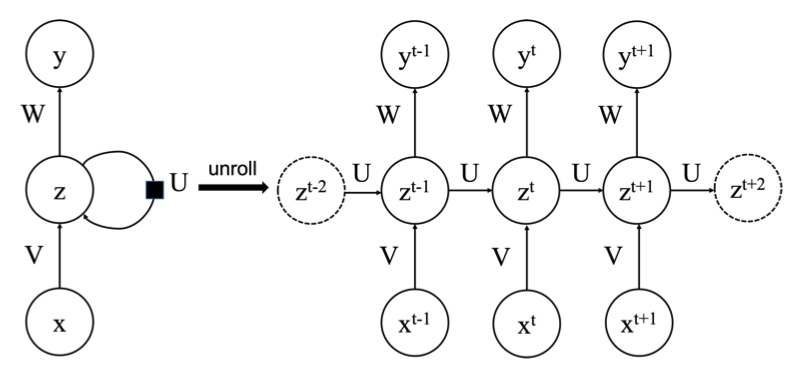
\includegraphics[width=.87\linewidth]{rnn_unrolled.png}

$F_\theta$ and $H_\varphi$ are parametrized as $F_{U,V}(\mathbf z, \mathbf x)=\phi(U\mathbf z+V\mathbf x)$ and $H_W(\mathbf z)=\psi(W\mathbf z)$ for activation functions $\phi, \psi$.
 
\textbf{Backpropagation (through time)}:

\resizebox{\linewidth}{!}{Propagation: $\color{teal}\frac{\partial z^{k+1}}{\partial z^{k}} \!=\! \frac{\partial \phi(U z^k + V x^{k+1})}{\partial z^{k}} \!=\! diag(\dot \phi(U z^k + V x^{k+1})) U$}

\hspace{47pt} $\color{blue}\frac{\partial y^s}{\partial z^s} = \frac{\partial \psi(W z^s)}{\partial z^{s}} = diag(\dot \psi(W z^s)) W$

Per State: $\color{violet}\frac{\partial E}{\partial z^q} = \sum_{s=q}^T \frac{\partial E}{\partial y^s} \frac{\partial y^s}{\partial z^q} = \sum_{s=q}^T \frac{\partial E}{\partial y^s} {\color{blue}\frac{\partial y^s}{\partial z^s}} \prod_{k=q}^{s-1} \color{teal}\frac{\partial z^{k+1}}{\partial z^k}$

$\bullet \frac{\partial E}{\partial W} = \sum_{s=1}^T \frac{\partial E}{\partial y^s} \frac{\partial y^s}{\partial W} = \sum_{s=1}^T (\Dot{\psi}(Wz^s) \odot z^s) \frac{\partial E}{\partial y^s}$

$\bullet \frac{\partial E}{\partial U} \!=\! \sum_{q=1}^T {\color{violet}\frac{\partial E}{\partial z^q}} \frac{\partial z^q}{\partial U} \!=\! \sum_{q=1}^T (\dot\phi(Uz^{q\text{-}1}+Vx^{q}) \odot z^{q\text{-}1}) {\color{violet}\frac{\partial E}{\partial z^q}}$

$\bullet \frac{\partial E}{\partial V} \!=\! \sum_{q=1}^T {\color{violet}\frac{\partial E}{\partial z^q}} \frac{\partial z^q}{\partial V} \!=\! \sum_{q=1}^T (\dot\phi(Uz^{q\text{-}1}+Vx^{q}) \odot x^{q}) {\color{violet}\frac{\partial E}{\partial z^q}}$
\\

$\bullet \color{purple}\frac{\partial E}{\partial \theta} = \sum_{t=1}^T \!\!\frac{\partial E}{\partial y_t} \frac{\partial y_t}{\partial z_t} \sum_{i=1}^t\!( \prod_{k=t}^{i+1} \!\frac{\partial z_k}{\partial z_{k-1}}) \frac{\partial F_\theta(z,x)}{\partial \theta} \big\vert_{z=z^{i-1}\!\!, x = x^{i-1}}$

\textbf{Exploding/Vanishing Gradients}:\\ 
$\norm{A}_2=\max_{x:\norm{x}=1}\norm{Ax}_2=\sigma_1(A) \hfill \norm{AB}_2\leq \norm{A}_2\norm{B}_2$\\
In backpropagation the following derivative occurs:\\
$\frac{\partial z^T}{\partial z^0}=\dot{\Phi}^TU\cdots \dot{\Phi}^1U$ where $\dot{\Phi}^t=\text{diag}(\dot \phi (Uz^{t-1}+Vx^t))$ and $\exists \alpha : $ $\dot{\Phi}^t\leq\alpha I$ (RELU: $\alpha=1$, Sigmoid: $\alpha=1/4$). If $\sigma_1(U)<1/\alpha$, $\norm{\frac{\partial z^T}{\partial z^0}}_2\leq (\alpha\sigma_1(U))^T\rightarrow 0$ as $T\rightarrow \infty $ giving vanishing gradients. Similarly, exploding gradients occur.

\textbf{Bi-Directional RNN}:\\
Additionally evolve $\Tilde{z}^t=\phi(\Tilde{U}\Tilde{z}^{t+1}+\Tilde{V}x^t)$ with $\Tilde{z}^{T+1}=0$. Modified output map couples the two: $y^t=\psi(Wz^t+\Tilde{W}\Tilde{z}^t)$.

\textbf{Deep RNN/Stacked RNN/Hierarchical RNN:}\\ 
$z^{t,l}=\phi(U^lz^{t-1,l}+V^lz^{t,l-1})$ where $l$ denotes the layer and $z^{t,0}=x^t$. Output computed from last state $y^t=\psi(Wz^{t,L})$.

\subsection*{Gated Memory Units}
\textit{Addressing the problem of vanishing/exploding gradients}\\
Gating unit: $z_{gated} =\sigma(G\zeta)\odot z$ where $\sigma(\cdot) \in [0,1]$. Gating units are embedded into gated units (LSTMs or GRUs).\\

\textit{We neglect bias terms in the following.}\\
\textbf{Long-Short-Term-Memory Unit (LSTM) - 3 Gates}\\
\begin{minipage}{0.5\linewidth}
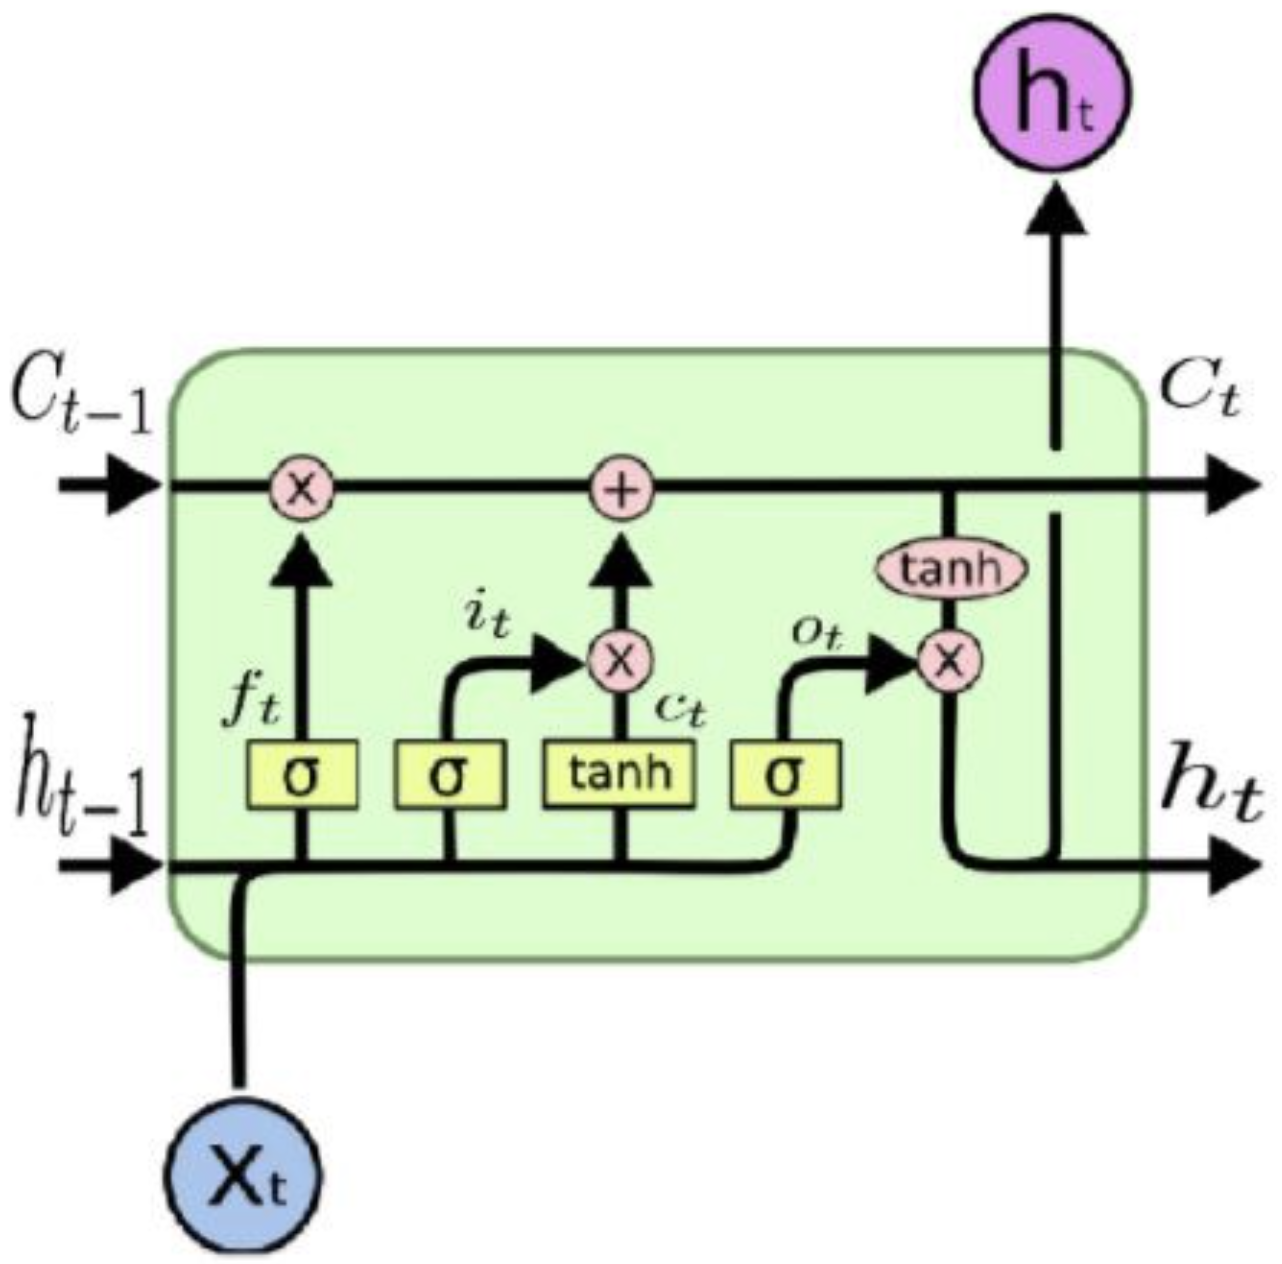
\includegraphics[width=\linewidth]{lstm_cell.png}
\end{minipage}
\begin{minipage}{0.5\linewidth}
    Augmented Input:\\
    $\tilde{x}_t = [h_{t-1}, x_t]$\\

    Output Gate:\\
    $h_{t} = \sigma(H \tilde{x}_{t}) \otimes \tanh(U C_{t})$\\
    
    Forget \& Input Gate:\\
    $C_t = \sigma(F \tilde{x}_t) \odot C_{t-1}$
    
    \hspace{8pt} $+\ \sigma(G \tilde{x}_t) \odot \tanh(V \tilde{x}_t)$\\

    Output Processing:\\
    $y_t = W h_t$
\end{minipage}
\underline{3} gating weight matrices: $H, F, G$, \underline{2} propagation weight matrices $U,V$, and \underline{1} output weight matrix $W$. \underline{6} in total. \\
\textbf{Gated Recurrent Unit (GRU) - 2 Gates}\\
\textit{Introduced to simplify LSTMs (less gates, less weights). The forget gate and input gate are convexly combined and the context cell/hidden state duality is removed.}\\

\begin{minipage}{0.5\linewidth}
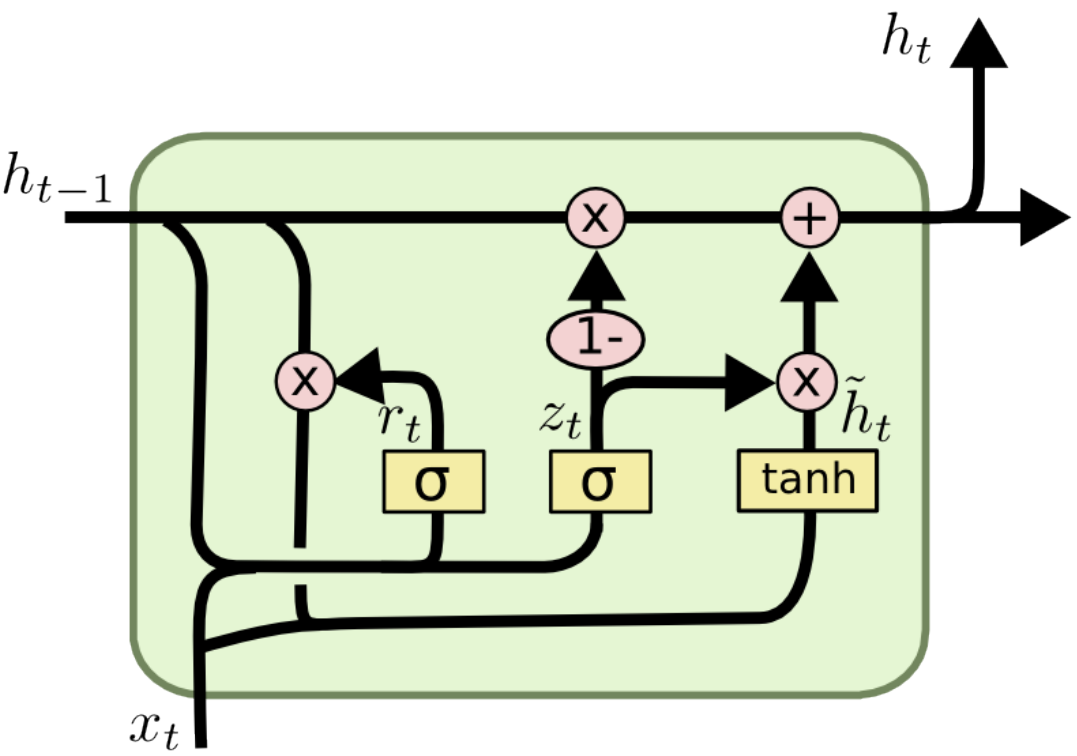
\includegraphics[width=\linewidth]{gru.png}
\end{minipage}
\begin{minipage}{0.5\linewidth}
Reset Gate:\\
$r_t = \sigma(H [h_{t-1}, x_t])$\\[-2pt]

Proposed Input:\\
$\tilde{h}_t = \tanh(V[r_t \odot h_{t-1}, x_t])$\\[-2pt]

Update Gate (Forget\&Input):\\
\resizebox{\linewidth}{!}{$h_t = (1\text{-}\sigma(G[h_{t\text{-}1}, x_{t\text{-}1}])) \odot h_{t\text{-}1}$}

\hspace{7pt} $+\ \sigma(G[h_{t\text{-}1}, x_{t\text{-}1}]) \odot \tilde h_t$\\[-2pt]

Output Processing\\ $y_t = W h_t$
\end{minipage}
\underline{2} gating weight matrices: $H, G$, \underline{1} propagation weight matrix $V$, and $1$ output weight matrix $W$. \underline{4} in total.

\subsection*{Linear Recurrent (State-Space) Models}
Linear state space model: $z^{t+1}=Az^t+Bx^t$ with diagonalization $A=P\Lambda P^{-1}$ over $\mathbb{C}$. Change of basis leads to $\zeta^{t+1}=\Lambda\zeta^t+Cx^t$ with $\zeta^t=P^{-1}z^t$ in complex state space ($\max_j\abs{\lambda_j}\leq 1$ for stabilization). To ensure high representational power of these systems, we give enough modelling power to the output map $y^t=\text{MLP}(\text{Re}(G\zeta^t))$.

\subsection*{Causal ($y^t \perp x^s\ \forall s > t$) Seq2Seq Modelling via RNN}
To learn $p(\mathbf y^{1:T}\mid \mathbf x^{1:T})\approx \prod_{t=1}^Tp(\mathbf y^t\mid \mathbf x^{1:t}, \mathbf y^{1:t-1})$ parametrize $p(y^t | x^{1:t}, y^{1:t-1})$ through $x^{1:t} \overset{F}{\mapsto} z^t \overset{H}{\mapsto} \mu^t \mapsto p_{\mu^t}(y^t)$. By introducing feedback links from $y^{t-1} \to z^t$ we can ensure that $z^t$ incorporates all knowledge on $x^{1:t}, y^{1:t-1}$.

\textbf{Teacher Forcing:}\\
\underline{During training}, compute loss on predicted output but feed back in actual output. \\
\underline{During prediction}, feed back predicted outputs. Improves learning BUT gives exposure bias (model only learns step predictions). \\
\underline{Professor Forcing} is a variant of teacher forcing that randomizes whether to feed back in $y_{pred}$ or $y_{true}$.\\
\textbf{Encoder-Decoder Model:} \\[2pt]
Encoder: $(\mathbf x^1,...,\mathbf x^T)\mapsto \mathbf z, \quad \mathbf z=\mathbf z^T$ (RNN)\\
Decoder $\mathbf z\mapsto (\mathbf y^1,...,\mathbf y^S)$ (RNN with output feedback)
\newcolumn

\section*{Attention}
\color{black}
\textit{Generate contextualised embeddings $\xi^s \in \mathbb{R}^m$ using convex combination of projected simple embeddings $x \in \mathbb{R}^e$:}

\hspace{3pt} $\xi^s = \sum_t a_{st} W x^t, \quad a_{st} \geq 0, \quad \sum_t a_{st} = 1$ with $\Xi = AXW^T$\\ 

\subsection*{Transformer Architecture \hfill $X \in \mathbb{R}^{L \times e}$}
\resizebox{\linewidth}{!}{$Q = X U_Q,\, K = X U_K,\, V = X U_V$ with $U_Q, U_K \in \mathbb{R}^{e \times d}, U_V \in \mathbb{R}^{e \times e}$}\\
\underline{Single-head:} $Attention(Q, K, V) = softmax(\tfrac{QK^T}{\sqrt{d}}) V$\\
\underline{Multihead:} $Multihead(Q,K,V) = Concat(H_1, \dots, H_h)W^O$

\hfill with $H_i= Attention(XU_Q^i, XU_K^i, X U_V^i)$ where

\hfill ${U_{\{Q,K\}}^i} \in \mathbb{R}^{n\times d_k}, U_V^i \in \mathbb{R}^{e \times d_v}, W^O \in \mathbb{R}^{hd_v\times e}$

\begin{minipage}{0.5\linewidth}
\textbf{Sinusoidal Pos. Encodings:}\\
For position $t$ and feature $k$:\\ $p_{tk}=\begin{cases} \sin(t\omega_k) \quad k \text{ even} \\ \cos(t\omega_k) \quad k \text{ odd} \end{cases}\\ \hfill \text{where } \omega_k=C^{k/n}, C=10000$\\

\textbf{Self-Attention:}
$Q,K,V$ from same sequence\\

\textbf{Cross-Attention:}
$Q$ from decoder, $K,V$ from encoder\\

\textbf{Masked Attention:}
Causal mask prevents peeking
\end{minipage}
\begin{minipage}{0.5\linewidth}
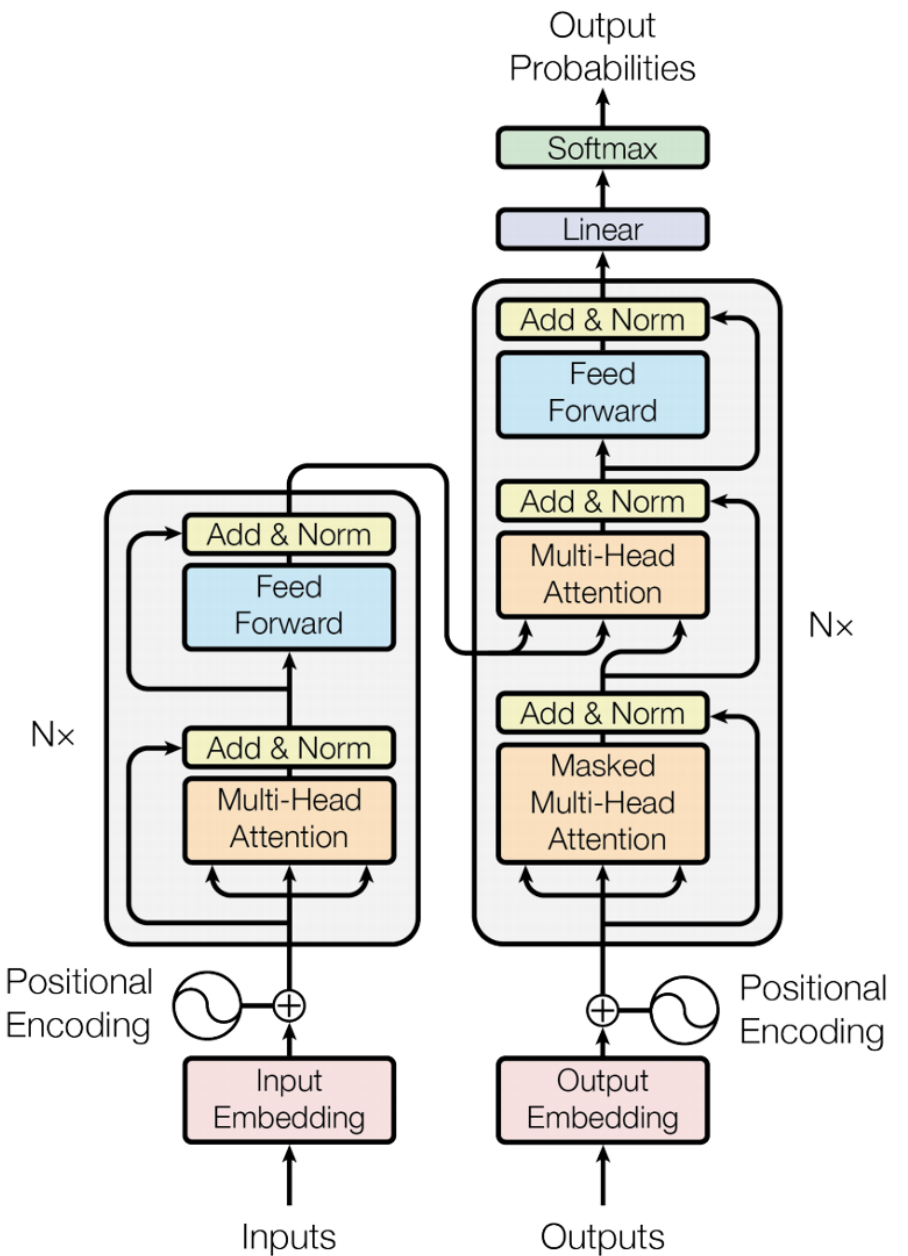
\includegraphics[angle=0, width=\linewidth]{transformer.png}\\
\end{minipage}

\textbf{RNN:} intelligent forgetting (compression)

\textbf{Transformer:} store and index intelligently\\


\subsection*{Memory Networks}
\textit{Recurrent attention model over external memory.}\\
\textbf{Recursive Associative Recall:} Given query $\mathbf q$ (e.g. question), find best matching memory cell $i$ and use its content $\mathbf m_i$ and $\mathbf q$ to generate new query - repeat
\subsection*{Applications in NLP}
\textbf{SpeechToText:} Easier to model $\mathbb P(speech | text)$ and use LLM for $\mathbb P(text)$ in $\mathbb P(text|speech) \propto \mathbb P(speech | text) \mathbb P(text)$.

\textit{Construct word embeddings that reflect the context}\\
\textbf{ELMo}: Contextualised word embeddings by stacking single CNN with bidirectional LSTMs. The contextualised embedding is derived from a parametrized convex combination of the hidden states across layers.\\
\textbf{BERT}: Bidirectional masked LLM. Pretrained by cloze task, i.e. predict masked word in text (word $\gets$ [MASK], random, or word), and by next sentence prediction, with input format \underline{[CLS], sentence A, [SEP], sentence B}. BERT is often fine-tuned for specific downstream task.\\
\textbf{GPT-n}: (Autogressive decoder model) Few, one, or zero shot learning (no gradient updates) - add task description \& examples to working memory and predict.\\
\textbf{Vision transformers}: Use vectorised image patches as ''word'' embeddings for Transformer (encoder).
\color{red}

\color{black}
\section*{Statistical Learning Theory}
\textit{Uniform general bounds given function class \(\mathcal F\) (DNN).}
\resizebox{\linewidth}{!}{\textbf{Shatter Coef.:} $S(\mathcal{F}, s) = \underset{x_1, \ldots, x_s}{\max} |\{(f(x_1), \ldots, f(x_s)) \in \{\pm 1\}^s\ | f \in \mathcal{F}\}|$}

\textbf{VC dimension:} $\max \{s : S(\mathcal{F}, s) = 2^s\} \leq \log_2 |\mathcal{F}|$

\resizebox{\linewidth}{!}{\textbf{VC inequ.:} 
$\mathbb P [\sup_{f \in \mathcal F} |\hat{R}_s(f) - R(f)| > \epsilon ] \leq 8 S(\mathcal{F}, s) e^{-s \epsilon^2 / 32}$}
A finite VC dimension is required for non-trivial bound.

\textbf{Change Of Measure Inequality:}\\
$\mathbb E_Q Z \leq KL(Q||P) + \ln \mathbb E_P e^Z \quad Q \ll P \quad Z \text{ is }P-\text{measurable}$

\textbf{PAC-Bayesian Theorem:}\\
\textit{Philosphy: $P$ anchors $Q$ ($P$ must not depend on any samples from $\mathcal{D}$, but $Q$ can) to ensure convergence/bound.}

Fix $P$ (prior) and $\mathcal{D}$ (data). Then for any $Q \ll P$ it holds with $\mathbb P_\mathcal{D}[\cdot] \geq 1-\epsilon$ that $\mathbb{E}_Q[ e_f - \hat e_f] \leq \sqrt{\frac{2KL(Q||P) + \ln \frac{2\sqrt{s}}{\varepsilon}}{s}}$\\
with true risk $e_f = \mathbb{E}_\mathcal{D} \mathds{1}_{f(x) \not = y}$, $s$-sample risk $\hat{e}_f = \mathbb{E}_{\mathcal{D}_s} \mathds{1}_{f(x) \not = y}$, and param distributions $Q, P$ over $f \in \mathcal F$.
\section*{Neural Tangent Kernel (NTK)}
CNNs can perfectly classify CIFAR-10 with random labels and permuted pixels (but no generalization to test).

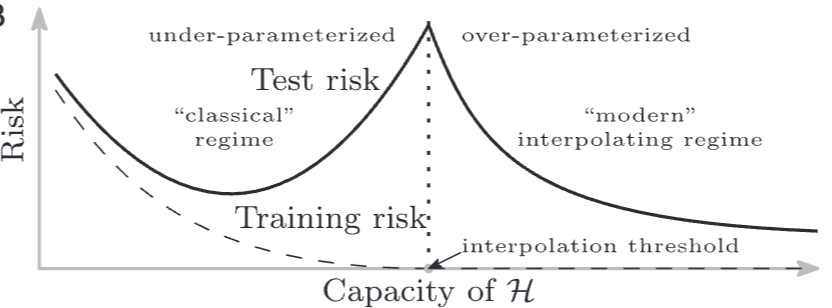
\includegraphics[width=\linewidth]{Deep-Learning-ETH-Summary-main/double_descent.png}

The NTK explains the interpolating regime, in particular why test accuracy decreases despite traing accuracy already being at 100\%. Assume a NN \(f : \mathbb{R}^d \times \mathbb{R}^n \to \mathbb R\).

\textbf{Neural Tangent Features:} \(\nabla_\theta f_\theta(x) \in \mathbb{R}^d\)\\
in analogy to generalized linear model \(f_\theta(x) = \theta^T \Phi(x)\)

\resizebox{\linewidth}{!}{\textbf{Neural Tangent Kernel (NTK):} $K_\theta(x,y) \!=\! \langle \nabla_\theta f_\theta(x), \nabla_\theta f_\theta(y) \rangle $}

\textbf{NTK Gram Matrix:} $K(\theta) \in \mathbb{R}^{s \times s}\quad K_{i,j}(\theta) = K_\theta(x_i, x_j)$

\textbf{Gradient Descent on sample $\{x_1, \ldots, x_s\}$ via NTK:}\\
Minimize \(\ell(\theta) = \frac{1}{2} \sum_{i=1}^s (f_\theta(x_i) - y_i)^2 \) via parameter gradient flow (ODE): \(\frac{d\theta}{dt} = - \nabla_\theta \ell(\theta) = \sum_{i=1}^s (y_i - f_\theta(x_i)) \nabla f_\theta(x_i)\).

\resizebox{\linewidth}{!}{\underline{Functional Gradient Flow:} $\frac{d f_\theta(x_j)}{dt} = \sum_{i=1}^s (y_i - f_\theta(x_i)) K_\theta(x_j, x_i)$}
which using the NTK Gram matrix gives $\frac{d \bf f}{dt} = K(\theta(t)) (\mathbf y - \mathbf f)$

\textbf{Linearize DNN around $\theta_0$ to get constant NTK $K_\theta = K$:}\\
$h(\vartheta)(x) = f_{\theta_0}(x) + \vartheta^T \nabla_\theta f_\theta(x) \vert_{\theta = \theta_0}  \quad \text{ where } \quad \vartheta = \theta - \theta_0$\\
Applying GD: $\vartheta \in \mathrm{span} \{\nabla_\theta f_\theta(x_1)|_{\theta=\theta_0}, \ldots, \nabla_\theta f_\theta(x_s)|_{\theta=\theta_0}\}$

\resizebox{\linewidth}{!}{Dual representation of minimizer: $\vartheta^* = \sum_{i=1}^s \alpha_i \nabla_\theta f_\theta(x_i)|_{\theta=\theta_0}$}

\resizebox{\linewidth}{!}{Loss function $\ell(\theta) = \frac{1}{2} \sum_{i=1}^s (\vartheta^T \nabla_\theta f_\theta(x_i)|_{\theta=\theta_0} - [y_i-f_{\theta_0}(x_i)])^2$}
Convex Kernel Regression: $\alpha^* = K^\dagger (\theta_0) (\bf y - \bf f_{\theta_0})$

Predict $f^*(x) = f_{\theta_0}(x) + K_{\theta_0}(x, (x_1, \ldots, x_s)) K^\dagger(\theta_0) (\bf y - \bf f_{\theta_0})$

\underline{DNN induces a random NTK whose Gradient Flow solu-}
\underline{tion approximates the optimal parameters to wide DNNs.}

\textbf{Nonlinear Deep Networks with constant NTK:}\\
Init $w_{ij}^l \sim \mathcal{N}(0,  \frac{\sigma_w^2}{m_l}), b_i^l \sim \mathcal{N}(0, \frac{\sigma_b^2}{m_l})$ at layer \(l\) with width \(m_l\).\\
In the infinite width limit \(m_l \to \infty\), $K_{\theta_0} \to K$ in probability, where $K$ depends on the model architecture and \(\sigma_w, \sigma_b\).

\underline{NTK Constancy}: In the $\infty$-width limit $\frac{d K_{\theta_t}}{dt} = 0$. We get a kernel machine 
$f^*(x) = f_{\theta_0}(x) + K(x, (x_1, \ldots, x_s)) K^\dagger (\bf y - \bf f_{\theta_0})$.
\underline{Emergence of constancy:} $\frac{||\nabla^2_\theta f_{\theta_0}(x)||_2}{||\nabla_\theta f_{\theta_0}(x)||_2^2 } \ll 1$ in the $\infty$-limit. Empirically, $||K(\theta_0) - K(\theta_t)||_F \in \mathcal{O}(\frac{1}{\sqrt{m}})$ over bounded \(\mathcal X\).
\section*{DNNs as Gaussian Processes}
Given a linear layer \(F:\mathbb{R}^n \to \mathbb{R}^m\quad x \mapsto Wx\) with weights \(w_{ij} \sim \mathcal{N}(0, \frac{\gamma^2}{n})\) and given \(X = [x_1, \ldots, x_s]\) one gets the GP \(WX \sim \mathcal{N}(0, K)\) with \(K_{i\mu, j\nu} = \mathds{1}_{i=j}\frac{\gamma^2 \langle x_\mu, x_\nu \rangle}{n}\). In a DNN the l'th layer preactivation \(W^l X^{l-1}\) is not normal ($X^{l-1}$ is random). In the wide layer limit the CLT restores a GP for preactivations whose \(K\) can be computed recursively (numerically): $K_{i \mu, j \nu}^l = \mathds{1}_{i=j} \mathbb{E}[\sum_s w_{is}\phi(x_{s\mu}^{l-1}) \sum_t w_{it}\phi(x_{t\nu}^{l-1})]$ where $x^{l-1} \sim GP(0, K^{l-1})$ and $\phi$ denotes the activation function. The preactivation Gaussian Process of the output layer can then be conditioned for prediction with conditional mean $f^*(x) = k(x, (x_1, \ldots, x_s)) K^\dagger y$ and variance $k^*(x,x) = k(x,x) - k(x, (x_1, \ldots, x_s)) K^\dagger k(x, (x_1, \ldots, x_s))^T$.

\section*{Sampling from Posterior for Bayesian DNNs}

\textbf{Markov Chain Monte Carlo:}
Gibb's distribution: \(p(\theta|\mathcal{D}) =\! \tfrac{1}{Z}\! \exp(-f(\theta))\) \resizebox{.755\linewidth}{!}{with energy function \(f(\theta) \!=\! -\log p(\theta|\mathcal{D}) \!-\! \log Z\)}.\\
In Metropolis Hastings with proposal distribution \(r(\theta'|\theta)\) we accept with $\mathbb{P}[accept] \!=\! \mathrm{min}\{1,\!\tfrac{r(\theta|\theta')}{r(\theta'|\theta)}\! \exp(f(\theta)\!-\!f(\theta'))\}$.

\textbf{Hamiltonian Monte Carlo visits all modes of posterior:}\\
Lift \(p(\theta | \mathcal{D})\) to \(p(\theta,y | \mathcal{D}) \propto \exp(-H(\theta,y))\) with momentum \(y\) and \(H(\theta,y) = ||y||_2^2 / 2m + f(\theta)\). Sample 
$p(y|\theta, \mathcal{D}) \sim \mathcal{N}(0, mI)$ and simulate for some \(\Delta t\) \(\tfrac{d\theta}{dt} = \nabla_y H \quad \tfrac{dy}{dt} = - \nabla_\theta H\) with \resizebox{\linewidth}{!}{acceptance probability \(\min(1, \exp(H(\theta,y) - H(\theta',y'))) =  1\).} If \resizebox{\linewidth}{!}{$\nabla_\theta H$ is estimated stochastically, acceptance is not guaranteed.}
\resizebox{\linewidth}{!}{We can add friction and noise (\underline{Langevin dynamics}) to $\frac{dy}{dt}$:}

\hspace{35pt} $dy = - \nabla_\theta H\ dt - \underset{\mathrm friction}{B\ y\ dt} + \underset{noise}{\mathcal{N}(0, 2B \ dt)}$
\section*{Model Distillation}
Parameters are an incomplete description of a network. Sampling of input/output map is most efficient for processing of model architecture. For better gradients a \underline{tempered softmax} (temperature > 1) recovers more information from the teacher (cross-entropy loss alignment).

\color{red}
\color{black}
\section*{Adversarial Robustness}
\textit{Adversarial examples are small manipulations of input which cause the model to change its prediction.}\\
\subsection*{Unconstrained Perturbations - DeepFool}
\textit{Smallest perturbation in $l_p$-norm that induces mistake, detectable since close to decision boundary.}\\

Given a linear multiclass model $g(x) = \arg \max_i f_i(x)$ where $ f_i = w_i^T x + b_i$ the $||\cdot||_2$-optimal perturbation is given by the smallest norm $\eta_i = \frac{f_{true}(x) - f_i(x)}{||w_{true} - w_i||_2^2} (w_i - w_{true})$. By linearization of a DNN we can iterate (DeepFool): repeatedly

\resizebox{\linewidth}{!}{$\min_{i, \nabla\eta} ||\nabla\eta||_2$ s.t. $(\nabla f_{true}(x) - \nabla f_i(x))^T \nabla \eta + f_{true}(x) -  f_i(x) < 0$}

\subsection*{Robust Training using Constrained Perturbations}
\textbf{Loss:} $\ell_{robust}^\epsilon(f_\theta(x), y) = \max_{\eta : ||\eta||_p \leq \epsilon} \ell(f_\theta(x+\eta), y)$ where the maximization can be solved by projected gradient ascent with projectors $\Pi_p z = \epsilon z/||z||_p$. For $p=2$ the gradient steps use $\nabla_x \ell$ and for $p=\infty$ they use $\text{sign}\nabla_x \ell$ instead.
\resizebox{\linewidth}{!}{\textbf{FastGradientSignMethod:} $p=\infty$ and single step with $\text{lr} = 1$.}
\color{black}
\section*{Generative Models}
\textbf{1 - Prescribed Model}: Density explicitly specified $p_\theta(x|z)$\\
which needs integration \(p_\theta(x) = \int_z p_\theta(x|z) p(z) dz\).

\textbf{2 - Implicit Model}: Directly generate data $x = f_\theta(z)$,\\
with implicit distribution $p_\theta(x) = p_z(f_\theta^{-1}(x)) |\frac{df_\theta^{-1}(x)}{dx}|$.\\
\textbf{Mode Collapse:} $\exists x : p(x) \gg p_\theta(x) \approx 0$\\
\textbf{False Generation:} $\exists x : p_\theta(x) \gg p(x) \approx 0$\\
\color{black}
\section*{Autoregressive Models}
\resizebox{\linewidth}{!}{Generate output one variable at a time based on chain rule:}\\
\resizebox{\linewidth}{!}{$p(x_1, \ldots, x_m) = \prod_{t=1}^m p(x_t | x_{1:t-1})$. Used in LLMs/PixelCNN/WaveNet.}


\section*{Autoencoders}
\subsection*{Linear Autoencoder}
\textbf{Def:} $\mathbf{x\mapsto z \mapsto y}, \quad \mathbf{z=Cx, \ y=Dz, \quad C,D}^T\in\mathbb R^{m\times n}, m<n$\\
\textbf{Loss:} $\ell(\mathbf x)=\frac{1}{2}||\mathbf{x-y}||^2 =\frac{1}{2}||\mathbf{x-DC x}||^2$\\
\textbf{Matrix notation:} $\mathbf{X,Y}\in\mathbb{R}^{n\times s}:\ \min_{D,C}\frac{1}{2s}||\mathbf{X-DCX}||^2_F$\\
\resizebox{\linewidth}{!}{\textbf{Eckhart-Young-Mirsky: } $\min_{\text{rank}(\mathbf Y)\leq r}||\mathbf{X-Y}||_F = ||\mathbf{X-X}_r||_F$}\\
for $X = U \Sigma V^T$ set $\mathbf{C=U}_m^T, \mathbf{D=U}_m \Rightarrow \mathbf{DCX=X}_m$

\subsection*{Linear Factor Analysis}
\textbf{Latent variable prior:} $\mathbf z\sim\mathcal N(\mathbf 0,\mathrm I), \quad \mathbf z\in\mathbb R^m, \quad m \ll n$\\
\textbf{Linear observation model:} $\mathbf x=\pmb\mu+\mathbf{Wz}+\pmb\eta \in\mathbb R^n$ where

\hfill $\pmb\eta\sim\mathcal N(\mathbf 0, \pmb\Sigma),\ \pmb\Sigma:=\text{diag}(\sigma_1^2,...,\sigma_n^2)$ $\Rightarrow$ $\mathbf x\sim\mathcal N(\pmb\mu,\mathbf{WW}^T+\pmb\Sigma)$\\
\textbf{Non-identifiability:} $(\mathbf{WQ})(\mathbf{WQ})^T=\mathbf{WW}^T$ for $\mathbf Q \in O(m)$\\
\textbf{Posterior inference:} \hfill $\pmb\mu_{\mathbf{z|x}}=\mathbf W^T(\mathbf{WW}^T+\pmb\Sigma)^{-1}(\mathbf x-\pmb\mu)$

\hfill $\pmb\Sigma_{\mathbf{z|x}}=\mathbf I-\mathbf W^T(\mathbf{WW}^T+\pmb\Sigma)^{-1}\mathbf W$\\
\textbf{MLE:} $\max_{\mu, W}\log p(\mathbf X;\pmb\mu,\mathbf W)$, has no closed form solution\\
\textbf{Probabilistic PCA}: for $\pmb\Sigma=\sigma^2\mathbf I$, $w_i^* = \sqrt{\max(0, \lambda_i - \sigma^2)} \cdot u_i$
with $(\lambda_i, u_i)$ the i'th eigenvalue/-vector of $X X^T \in \mathbb{R}^{n \times n}$.
\subsection*{Variational Autoencoders}

Latent variable $\mathbf z\sim\mathcal N(\mathbf 0, \mathbf I)$ and conditional $p_\theta(x|z)$ require intractable integration for $p_\theta(x)$ (MLE). Hence, we max.\\
\textbf{ELBO:} $\log p(\mathbf x;\pmb\theta)\geq \mathbb E_{\mathbf z\sim q(\mathbf z;\mathbf x)}[\log p(\mathbf x|\mathbf z;\pmb\theta)]-\text{D}(q(\mathbf z;\mathbf x)||p(\mathbf z))$

\hfill $= \log p(\mathbf x;\pmb\theta) - \text{D}(q(\mathbf z;\mathbf x)||p(\mathbf z | \mathbf x, \pmb \theta))$


$q(\mathbf z;\mathbf x)$ is restricted to (typic. Gaussian) variational family: \\ $\mathcal N(\mathbf z;\pmb\mu(\mathbf x),\pmb\Sigma(\mathbf x)), \text{ where } \pmb\Sigma(\mathbf x)=\text{diag}(\sigma_1^2(\mathbf x),...,\sigma_n^2(\mathbf x))$\\
stochastic backpropagation / re-parameterization trick:\\
$\mathbf z\sim\mathcal N(\pmb\mu(\bf x),\pmb\Sigma(\bf x)) \quad \Leftrightarrow \quad\mathbf z=\pmb\mu(\bf x)+\pmb\Sigma^{1/2} \bf(x)\ \pmb\eta, \quad \pmb\eta\sim\mathcal N(\mathbf 0,\mathrm I)$


\section*{Normalizing Flows}
Implicit model $f_\theta(z)$ with tractable $f_\theta^{-1}(x)$ and $\det \frac{d f_\theta^{-1}(x)}{d x}$. Restrict $f_\theta$ to $C^1$-diffeomorphisms by having each $F_j$ in
$f_\theta=F_L\circ\cdot\cdot\cdot\circ F_1$ be one with specified $F_j^{-1}$ and $\det(\partial F_j)$:\\
\resizebox{\linewidth}{!}{$f_\theta^{-1}=F^{-1}_1\circ\cdot\cdot\cdot\circ F_L^{-1} \land  \text{det}\frac{df_\theta^{-1}(x)}{dx}=\prod_{l=L}^1\text{det}\partial F_l^{-1}\circ F_{l+1:L}^{-1}(x)$}\\
\resizebox{\linewidth}{!}{Flows are universal and optimised via gradient descent of}

$D(p^*||p_\theta) + H(p^*) = \mathbb E_{p^*}[- \log p_z(f_\theta^{-1}(x)) - \log | \det \frac{d f_\theta^{-1}(x)}{d x}|]$
\textbf{Linear Flow}: $F_j(\mathbf x)=\mathbf{A_jz+b_j}$. Set $A_\theta = Q_\theta R_\theta$ for efficient $A^{-1}(x)$ in $\mathcal{O}(n^2)$ and $|\det A|$ in $\mathcal{O}(n)$ instead of both in $\mathcal{O}(n^3)$.\\
\textbf{Autoregressive Flow:} $x_i = \tau(z_i; c_i(z_1, \ldots, z_{i-1}))$ where $z \mapsto \tau(z;h)$ is strict monotonous with arbitrary conditioner $c_i$. Closely related to Linear Flows one gets efficient $\tau^{-1}(x)$ and $\det \partial \tau$ with upper diagonal Jacobian $\partial \tau$. 

\textbf{Invertible Linear Time Flows}: $F_j(\mathbf z)=\mathbf z+\mathbf u\sigma(\mathbf{\langle w, z\rangle}+b)$ \\

\color{red}


\color{black}
\columnbreak

\section*{Generative Adversarial Networks (GANs)}
\textit{Derive training signal for generator $G_\theta$ from classifier $D_\phi$ that discriminates data from model-generated samples.}\\
\textbf{Shared Data Generation:} $\tilde p_\theta(\mathbf x, y)=\frac{1}{2}(yp(\mathbf x)+(1-y)p_\theta(\mathbf x))$\\
\resizebox{\linewidth}{!}{\textbf{Objective:} $\ell(\theta, \phi) = \frac{1}{2}\mathbb{E}_p[\log(q_\phi(x))] + \frac{1}{2}\mathbb{E}_{p_\theta} [\log(1-q_\phi(x))]$}\\
\textbf{Optimal Discriminator:} $q_\theta(\mathbf x)=\frac{p(\mathbf x)}{p(\mathbf x)+p_\theta(\mathbf x)}=\tilde P_\theta(y=1|\mathbf x)$\\
\textbf{Objective given $q_\phi(x) \equiv q_\theta(x)$ becomes JS-divergence:}\\
\resizebox{\linewidth}{!}{$\ell(\theta, \phi^*)\!+\!\log 2 \!=\! \underset{\substack{anti-mode-\\collapse}}{\frac{1}{2}D(p||\frac{p\!+\!p_\theta}{2})} + \underset{\substack{anti-false-\\generation}}{\frac{1}{2}D(p_\theta || \frac{p\!+\!p_\theta}{2})} \!=\!\underset{\in [0, \log 2]}{\text{JSD}(p,p_\theta)}$}
\resizebox{\linewidth}{!}{\textbf{Training difficulties ($k$ update steps on $D_\phi$ per step on $G_\theta$):}}\\
$k \gg 1 \Rightarrow$ Strong discriminator $\Rightarrow$ vanishing gradients\\
$k \approx 1 \Rightarrow$ Weak discriminator $\Rightarrow$ mode collapse
\subsection*{Wasserstein-GAN}
\textit{JS-divergence saturates if the support of $p_\theta, p$ does not overlap. Hence min. $W(p, p_\theta) \!=\! \inf_{\gamma \sim \Pi(p, p_\theta)} \!\mathbb{E}_{(x,y) \sim \gamma} ||x\text{-}y||.$}
2\textbf{KR-duality:} %Kantorovich-Rubinstein
$W(p, p_\theta) \!=\! \frac{1}{K} \sup_{||f||_L \leq K} \mathbb{E}_{p} f(x) - \mathbb{E}_{p_\theta} f(x)$\\
Parametrize discriminator $f = f_\phi$ where the $K$-Lipschitz condition can be enforced through weight clipping or gradient penalty $\mathbb E_{p_{\hat{x}}}[(||\nabla_{\hat{x}} f_\phi(\hat{x})||_2 - 1)^2]$ where $\hat{x}$ is sampled along straight lines between $x_1 \sim p$ and $x_2 \sim p_\theta$.
\section*{Diffusion Models}
\textbf{Noising:} $q(x_t | x_{t-1}) = \mathcal{N}(x_t ; \sqrt{1-\beta_t} x_{t-1}, \beta_t I)$, $\beta_t \in (0,1)$\\%$q(x_{1:T}|x_0) = \prod_{t=1}^T q(x_t | x_{t-1})$
\textbf{Shortcut Noising:} $q(x_t | x_0) = \mathcal{N}(x_t ; \sqrt{\bar \alpha_t} x_0, (1-\bar \alpha_t) I)$ where $\alpha_t = 1-\beta_t \in (0,1)$ and $\bar \alpha_t = \prod_{i=1}^t \alpha_i$ \textcolor{gray}{(proof by induction)}\\
\textbf{Convergence of Noising:} $\lim_{t\to\infty} q(x_t | x_0) = \mathcal{N}(\ \cdot\ ;0, I)$\\

\textbf{Denoising:} $q(x_{t-1} | x_t) = q(x_t | x_{t-1})\frac{q(x_{t-1})}{q(x_t)}$ is intractable, but Gaussian for $\beta_t \approx 0$, hence parametrize $p_\theta(x_{t-1} | x_t)$.

\textbf{Variational Lower Bound of Likelihood:}\\
$\log p_\theta (x_0) \geq \log p_\theta (x_0) - D_{KL}(q(x_{1:T}|x_0)|| p_\theta(x_{1:T} | x_0)) \!=\! $

\resizebox{\linewidth}{!}{$\text{-} \mathbb{E}_{q(x_{1:T}|x_0)} [\log \frac{q(x_{1:T}|x_0)}{p_\theta(x_{0:T})}] \!=\! \text{-} \mathbb{E}_{q(x_{1:T}|x_0)}[\underset{L_T}{D(q(x_T | x_0) || p_\theta(x_T))}$}

\hfill $+\sum_{t=2}^T \underset{L_{t-1}}{D(q(x_{t-1} | x_t, x_0) || p_\theta(x_{t-1} | x_t))} \underset{L_0}{- \log p_\theta(x_0 | x_1)} ]$

\textbf{Diffusion Loss Terms (minimized in $\mathbb{E}_{p(x_0)}\mathbb{E}_{q(x_{1:T}|x_0)}$):}

\resizebox{\linewidth}{!}{$\lim_{T\to\infty} L_T \!=\! D_{KL}(\mathcal{N}(\ \cdot\ ;0,I) || p_\theta(x_T)) \Rightarrow$ set $p_\theta(x_T) = \mathcal{N}(\cdot; 0, I)$.}\\
$L_0$ is often ignored in practice. That leaves $L_t$, where\\

$q(x_{t-1}|x_t, x_0) = \frac{q(x_0 | x_{t-1}) \cdot q(x_{t-1} |x_t)}{q(x_0 | x_t)} \approx \mathcal{N}(x_{t-1}; \tilde \mu(x_t, x_0), \tilde \beta_t I)$ \resizebox{\linewidth}{!}{with $\tilde{\mu}_t(x_t, x_0) = \frac{1}{\sqrt \alpha_t}(x_t - \frac{1-\alpha_t}{\sqrt{1-\bar\alpha_t}} \overset{= \epsilon_t}{\frac{x_t - \sqrt{\bar\alpha_t} x_0}{\sqrt{1-\bar\alpha_t}}})$, $\tilde \beta_t = \frac{1-\bar\alpha_{t-1}}{1-\bar\alpha_t} \beta_t$.}

\textbf{Parametrization:} $p_\theta(x_{t-1} | x_t) = \mathcal{N}(x_{t-1}; \mu_{\theta}(x_t, t), \tilde{\beta}_t I)$\\ 
where $\mu_\theta(x_t, t) = \frac{1}{\sqrt{\alpha_t}} (x_t - \frac{1-\alpha_t}{\sqrt{1-\bar \alpha_t}} \epsilon_\theta(x_t, t))$.

\textbf{Reparametrized Loss:}
$L_t = D_{KL}(q(x_{t-1} | x_t, x_0)||p_\theta(x_{t-1}|x_t))\\ = \frac{||\tilde \mu(x_t, x_0) - \mu_\theta(x_t, t)||^2}{2 \tilde \beta_t} %= \frac{(1-\alpha_t)^2 ||\tfrac{x_t - \sqrt{\bar\alpha_t}x_0}{\sqrt{1-\bar\alpha_t}} - \epsilon_\theta(x_t, t)||^2}{2 \alpha_t (1-\bar \alpha_t) \tilde\beta_t} 
= \frac{(1-\alpha_t)^2 ||\epsilon_t - \epsilon_\theta(\sqrt{\bar\alpha_t}x_0 + \sqrt{1-\bar\alpha_t}\epsilon_t, t)||^2}{2 \alpha_t (1-\bar \alpha_t) \tilde\beta_t}$

\textbf{In practice}, a simplified $L_{VLB}$ is minimized (SGD): $\mathbb{E}_{x_0 \sim p, t \sim \mathcal{U}([1,T]), \epsilon_t \sim \mathcal{N}(0, I)}[||\epsilon_t - \epsilon_\theta(\sqrt{\bar\alpha_t}x_0 + \sqrt{1-\bar\alpha_t}\epsilon_t, t)||_2^2$

\textbf{Generation:} Use $x_T \sim \mathcal{N}(0, I)$ and $x_{t-1} | x_t \sim p_\theta(x_{t-1} | x_t)$.

\textbf{Scheduler:} vital for performance. Slowly decrease $\bar \alpha_t$.


\columnbreak

\section*{Score-Based Models avoid Normalization}
\resizebox{\linewidth}{!}{\textit{Instead of learning $p(x)$, learn tractable \(\nabla \log p(x) = \frac{\nabla p(x)}{p(x)}\).}}
\textbf{Fisher Divergence loss:} $\ell(p,\theta) = \mathbb E_{p} ||\nabla_x \log p(x) - s_\theta(x) ||_2^2$

\hfill $= \mathbb E_p [||s_\theta(x)||_2^2 + 2 \text{Tr}( \nabla s_\theta(x) )] + C$

\textbf{Scaling:} $\ell(p,\theta) = \mathbb E_p \mathbb E_{v \sim \mathcal{U}(\mathcal{S}^d)}[(v^T\!\! s_\theta(x))^2 + 2 v^T\!\! \nabla s_\theta(x) v] + C$

\textbf{Sampling via ULA:} $x_{t+1} \sim \mathcal{N}(x_{t+1} ; x_t + \eta_t \nabla_x \log p(x), 2 \eta_t I)$

\textbf{Practical Issues:} \(s_\theta(x)\) only accurate where \(p(x) \gg 0\). Hence, adapt loss to
$\sum_{i=1}^L \lambda(i) \mathbb{E}_{p_{\sigma_i}}|| \nabla_x \log p_{\sigma_i} - s_\theta(x,i)||_2^2$ where $p_{\sigma_i}$ adds Gaussian noise to samples. 

\textit{The process of sampling (ULA) from \(S_\theta(x,i)\) where iteratively the noise is decreased is mathematically equivalent to sampling from a diffusion model (Inversion of SDE).}

\textbf{Forward SDE:} $dx = f(x,t) dt + g(t) dW$\\ 
\textbf{Reverse SDE:} $dx = f(x,t) dt - g^2(t) \nabla_x \log p_t(x) dt + g(t) dW$
\section*{Evaluation Metrics for Implicit Models}
\textit{Implicit Models cannot use evaluation likelihood score.}\\
\textbf{Inception Score:} $\exp(\mathbb E_{x \sim p_\theta} [KL(p(y|x)||\mathbb{E}_{x \sim p_\theta} p(y|x))])$ where $p(y|x)$ is given by InceptionV3. $p(y|x)$ should differ from marginal $p(y)$ which is achieved by confidence (no false generation) and coverage (no mode collapse).\\
\textbf{FID:} $||\mu - \mu_\theta||_2^2 + \text{Tr}(\Sigma + \Sigma_\theta - 2 (\Sigma \Sigma_\theta)^{1/2})$ where $\mu, \Sigma$ and $\mu_\theta, \Sigma_\theta$ are the empirical mean and covariance matrix of the InceptionV3 output layer based on real and generated images respectively. It corresponds to the Wasserstein distance between fitted m.v. Gaussians.
\section*{Python}
\subsection*{Basics}
Round to 2 Digits: {\color{blue} \verb|round(5.76543, 2)=5.77|}

List Comprehension: {\color{blue}\verb|[x**2 for x in list]|}

Conditionals: {\color{blue}\verb|result = val1 if cond else val2|}

\subsection*{Numpy ndarray Manipulation}
Determinant: {\color{blue}\verb|np.linalg.det(matrix)|}

Create Diagonal Matrix: {\color{blue}\verb|np.diag(diagonal_elements)|}

E-values, E-vectors $[v_1, \ldots, v_n]$: {\color{blue}\verb|np.linalg.eig(matrix)|}

Identity Matrix: {\color{blue}\verb|numpy.eye(size)|}

Inverse: {\color{blue}\verb|numpy.linalg.inv(matrix)|}

Frobenius/Eucl. Norm: {\color{blue}\verb|np.linalg.norm(vector/matrix)|}

Operator Norm:
{\color{blue}\verb|np.linalg.norm(matrix, ord=2)|}

Matrix Multiplication: {\color{blue}\verb|A @ B|}

SVD: {\color{blue}\verb|U,S,Vt = np.linalg.svd(matrix)|}

Trace: {\color{blue}\verb|np.trace(matrix)|}

Transpose: {\color{blue}\verb|A.getT() or A.transpose()|}

Element-wise Multiplication: {\color{blue}\verb|A * B|}

Element-wise Square Root: {\color{blue}\verb|np.sqrt(matrix)|}

Element-wise Exponential: {\color{blue}\verb|np.exp(matrix)|}

Element-wise logarithm: {\color{blue}\verb|np.log(matrix)|}

Matrix-Power:
{\color{blue}\verb|np.linalg.matrix_power(matrix, n)|}

\subsection*{Numpy Random ndarray Generation}
Uniform in $[0,1)$: {\color{blue}\verb|np.random.rand(rows, cols)|}

Int in $[low, high)$: {\color{blue}\verb|np.random.randint(low, high, size)|}

Normal Distr: {\color{blue}\verb|np.random.normal(mean, std_dev, size)|}

\subsection*{PyTorch Basics}

Autograd:
{\color{blue}
\verb|x=torch.tensor([1.0],requires_grad=True)|

\hfill \verb|y = x**2; y.backward(); gradient=x.grad|}

Forward pass: {\color{blue}\verb|model(torch.randn(1, 10))|}

Matrix Multiplication: {\color{blue}\verb|torch.mm(A, B)|}

Transpose: {\color{blue}\verb|A.t()|} or 

\hfill {\color{blue}\verb|torch.transpose(input, dim0, dim1)|}

\subsection*{Pytorch Neural Network Building Blocks}
{\color{blue}\verb|torch.nn.Module|}: base class for NN modules\\
{\color{blue}\verb|torch.nn.Linear|}: creates a fully connected layer

\subsection*{Pytorch Activation Functions}
{\color{blue}\verb|import torch.nn.functional as F|\\
\verb|output = F.relu(input), F.sigmoid(input), F.tanh(input)|}

\subsection*{Loss Functions}
{\color{blue}\verb|criterion = nn.MSE(), nn.CrossEntropyLoss(), nn.BCELoss|\\
\verb|loss = criterion(output, target)|}

\subsection*{Optimizers}
{\color{blue}\verb|optimizer = torch.optim.Adam(model.parameters(), lr=learning_rate)|\\
\verb|optimizer.zero_grad()|\\
\verb|loss.backward()|\\ \verb|optimizer.step()|}

\subsection*{Training Loop}
{\color{blue}\verb|for epoch in range(num_epochs):|\\
\verb|    for inputs, targets in dataloader:|\\
\verb|        optimizer.zero_grad()|\\
\verb|        outputs = model(inputs)|\\
\verb|        loss = criterion(outputs, targets)|\\
\verb|        loss.backward(); |\\
\verb|optimizer.step()|}

\newcolumn
\columnbreak
\vspace*{\fill}
\section*{Authors}
\textbf{Nicolas Menet, Jacky Choi, Chandra de Viragh,\\ Angéline Pouget, Leila Chettata}
\end{multicols*}
\end{document}